\documentclass[12pt]{article}
\usepackage[utf8]{inputenc}
\usepackage{amsmath}
\usepackage{breqn}
\usepackage{pgfplots}
\pgfplotsset{compat=1.18}
\usepackage{geometry}
\geometry{a4paper, left=20mm, right=20mm, top=20mm, bottom=20mm}
\setlength{\parindent}{0pt}
\setlength{\parskip}{1em}
\begin{document}
\begin{titlepage}
\centering
\vspace*{2cm}
{\Huge \textbf{Mathematical Expression Analysis}}\par
\vspace{1cm}
{\Large Automatic Differentiation and Optimization}\par
\vspace{2cm}
{\large Automatically generated report}\par
\vspace{1cm}
{\large \today}\par
\vfill
{\large Author: Patlasov Gregory Sergeevich}\par
\end{titlepage}

\vspace{1cm}
\section*{Introduction}
\addcontentsline{toc}{section}{Introduction}
This document presents a complete analysis of a mathematical expression, including:
\begin{itemize}
\item Original expression and its evaluation
\item Optimization and simplification process
\item \textbf{Lots of derivatives} of various orders
\item Variable table with their values
\end{itemize}
\newpage
\subsection*{Original Expression}
Expression:
\begin{dmath} \sin(x) + 5 \cdot x - (11 \cdot \ln(5 \cdot x + 7)) - 10000 + 10000 - 5000 + 10 \cdot 10 + 4914 \end{dmath}

Evaluation result:
\begin{dmath} -4.860347 \end{dmath}

\section*{Variable Table}
\begin{tabular}{|c|c|}
\hline
Name & Value \\
\hline
x & 3.0000 \\
\hline
\end{tabular}

\section*{Optimization}
Before optimization: \[ \sin(x) + 5 \cdot x - (11 \cdot \ln(5 \cdot x + 7)) - 10000 + 10000 - 5000 + 10 \cdot 10 + 4914 \]

\subsubsection*{Optimization Step}
It is easy to see that constant folding simplified part of expression to: 100.00:

\begin{dmath} \sin(x) + 5 \cdot x - (11 \cdot \ln(5 \cdot x + 7)) - 10000 + 10000 - 5000 + 100 + 4914 \end{dmath}

\vspace{0.5em}
\subsection*{Result optimization}
Final expression: \[ \sin(x) + 5 \cdot x - (11 \cdot \ln(5 \cdot x + 7)) - 10000 + 10000 - 5000 + 100 + 4914 \]

Final result: \[ -4.860347 \]

\section*{Graph of the Function}
\begin{figure}[h]
\centering
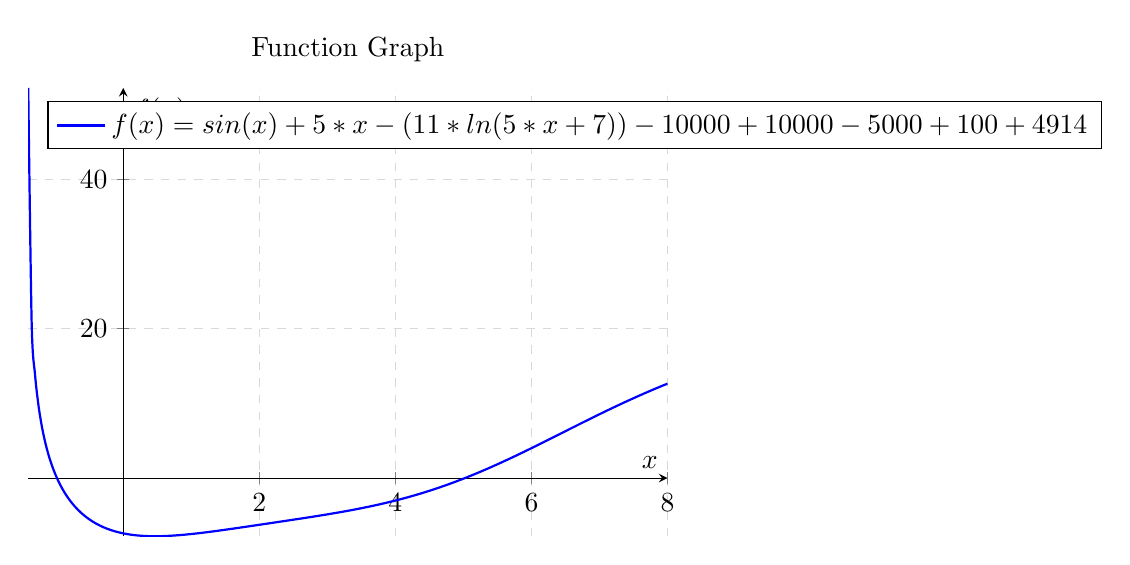
\begin{tikzpicture}
\begin{axis}[
    width=0.8\textwidth,
    height=0.6\textwidth,
    axis lines = middle,
    xlabel = {$x$},
    ylabel = {$f(x)$},
    grid = major,
    grid style = {dashed, gray!30},
    legend pos = north west,
    title = {Function Graph},
    domain = -2.000000:8.000000,
    samples = 200,
    trig format=rad
]
\addplot[blue, thick, smooth] {sin(x) + 5 * x - (11 * ln(5 * x + 7)) - 10000 + 10000 - 5000 + 100 + 4914};
\addlegendentry{$f(x) = sin(x) + 5 * x - (11 * ln(5 * x + 7)) - 10000 + 10000 - 5000 + 100 + 4914$}
\end{axis}
\end{tikzpicture}
\caption{Plot: $f(x) = sin(x) + 5 * x - (11 * ln(5 * x + 7)) - 10000 + 10000 - 5000 + 100 + 4914$}
\end{figure}
\vspace{1cm}
\section*{Differentiation}
Differentiation variable: \[ x \]

\subsection*{Optimization of derivative 1}
\section*{Optimization}
Before optimization: \[ \cos(x) \cdot 1 + 5 \cdot 1 + x \cdot 0 - (11 \cdot \frac{1}{5 \cdot x + 7} \cdot 5 \cdot 1 + x \cdot 0 + 0 + \ln(5 \cdot x + 7) \cdot 0) - 0 + 0 - 0 + 0 + 0 \]

\subsubsection*{Optimization Step}
It is easy to see that constant folding simplified part of expression to: 5.00:

\begin{dmath} \cos(x) \cdot 1 + 5 + x \cdot 0 - (11 \cdot \frac{1}{5 \cdot x + 7} \cdot 5 \cdot 1 + x \cdot 0 + 0 + \ln(5 \cdot x + 7) \cdot 0) - 0 + 0 - 0 + 0 + 0 \end{dmath}

\vspace{0.5em}
\subsubsection*{Optimization Step}
It is easy to see that constant folding simplified part of expression to: 5.00:

\begin{dmath} \cos(x) \cdot 1 + 5 + x \cdot 0 - (11 \cdot \frac{1}{5 \cdot x + 7} \cdot 5 + x \cdot 0 + 0 + \ln(5 \cdot x + 7) \cdot 0) - 0 + 0 - 0 + 0 + 0 \end{dmath}

\vspace{0.5em}
\subsubsection*{Optimization Step}
It is easy to see that mul one simplified:

\begin{dmath} \cos(x) + 5 + x \cdot 0 - (11 \cdot \frac{1}{5 \cdot x + 7} \cdot 5 + x \cdot 0 + 0 + \ln(5 \cdot x + 7) \cdot 0) - 0 + 0 - 0 + 0 + 0 \end{dmath}

\vspace{0.5em}
\subsubsection*{Optimization Step}
It is easy to see that mul zero simplified:

\begin{dmath} \cos(x) + 5 + 0 - (11 \cdot \frac{1}{5 \cdot x + 7} \cdot 5 + x \cdot 0 + 0 + \ln(5 \cdot x + 7) \cdot 0) - 0 + 0 - 0 + 0 + 0 \end{dmath}

\vspace{0.5em}
\subsubsection*{Optimization Step}
It is easy to see that adding zero simplified:

\begin{dmath} \cos(x) + 5 - (11 \cdot \frac{1}{5 \cdot x + 7} \cdot 5 + x \cdot 0 + 0 + \ln(5 \cdot x + 7) \cdot 0) - 0 + 0 - 0 + 0 + 0 \end{dmath}

\vspace{0.5em}
\subsubsection*{Optimization Step}
It is easy to see that mul zero simplified:

\begin{dmath} \cos(x) + 5 - (11 \cdot \frac{1}{5 \cdot x + 7} \cdot 5 + 0 + 0 + \ln(5 \cdot x + 7) \cdot 0) - 0 + 0 - 0 + 0 + 0 \end{dmath}

\vspace{0.5em}
\subsubsection*{Optimization Step}
It is easy to see that adding zero simplified:

\begin{dmath} \cos(x) + 5 - (11 \cdot \frac{1}{5 \cdot x + 7} \cdot 5 + 0 + \ln(5 \cdot x + 7) \cdot 0) - 0 + 0 - 0 + 0 + 0 \end{dmath}

\vspace{0.5em}
\subsubsection*{Optimization Step}
It is easy to see that adding zero simplified:

\begin{dmath} \cos(x) + 5 - (11 \cdot \frac{1}{5 \cdot x + 7} \cdot 5 + \ln(5 \cdot x + 7) \cdot 0) - 0 + 0 - 0 + 0 + 0 \end{dmath}

\vspace{0.5em}
\subsubsection*{Optimization Step}
It is easy to see that mul zero simplified:

\begin{dmath} \cos(x) + 5 - (11 \cdot \frac{1}{5 \cdot x + 7} \cdot 5 + 0) - 0 + 0 - 0 + 0 + 0 \end{dmath}

\vspace{0.5em}
\subsubsection*{Optimization Step}
It is easy to see that adding zero simplified:

\begin{dmath} \cos(x) + 5 - (11 \cdot \frac{1}{5 \cdot x + 7} \cdot 5) - 0 + 0 - 0 + 0 + 0 \end{dmath}

\vspace{0.5em}
\subsubsection*{Optimization Step}
It is easy to see that - 0 simplified:

\begin{dmath} \cos(x) + 5 - (11 \cdot \frac{1}{5 \cdot x + 7} \cdot 5) + 0 - 0 + 0 + 0 \end{dmath}

\vspace{0.5em}
\subsubsection*{Optimization Step}
It is easy to see that adding zero simplified:

\begin{dmath} \cos(x) + 5 - (11 \cdot \frac{1}{5 \cdot x + 7} \cdot 5) - 0 + 0 + 0 \end{dmath}

\vspace{0.5em}
\subsubsection*{Optimization Step}
It is easy to see that - 0 simplified:

\begin{dmath} \cos(x) + 5 - (11 \cdot \frac{1}{5 \cdot x + 7} \cdot 5) + 0 + 0 \end{dmath}

\vspace{0.5em}
\subsubsection*{Optimization Step}
It is easy to see that adding zero simplified:

\begin{dmath} \cos(x) + 5 - (11 \cdot \frac{1}{5 \cdot x + 7} \cdot 5) + 0 \end{dmath}

\vspace{0.5em}
\subsubsection*{Optimization Step}
It is easy to see that adding zero simplified:

\begin{dmath} \cos(x) + 5 - (11 \cdot \frac{1}{5 \cdot x + 7} \cdot 5) \end{dmath}

\vspace{0.5em}
\subsection*{Result optimization}
Final expression: \[ \cos(x) + 5 - (11 \cdot \frac{1}{5 \cdot x + 7} \cdot 5) \]

Final result: \[ 1.510008 \]

\subsection*{Derivative of Order 1}
Derivative:
\begin{dmath} f'(x) = \cos(x) + 5 - (11 \cdot \frac{1}{5 \cdot x + 7} \cdot 5) \end{dmath}

Value of derivative at point:
\begin{dmath} f'(x) = 1.510008 \end{dmath}

\subsection*{Optimization of derivative 2}
\section*{Optimization}
Before optimization: \[ -1 \cdot \sin(x) \cdot 1 + 0 - (11 \cdot \frac{1}{5 \cdot x + 7} \cdot 0 + 5 \cdot \frac{5 \cdot x + 7 \cdot 0 - (1 \cdot 5 \cdot 1 + x \cdot 0 + 0)}{5 \cdot x + 7 \cdot 5 \cdot x + 7} + \frac{1}{5 \cdot x + 7} \cdot 5 \cdot 0) \]

\subsubsection*{Optimization Step}
It is easy to see that constant folding simplified part of expression to: 5.00:

\begin{dmath} -1 \cdot \sin(x) \cdot 1 + 0 - (11 \cdot \frac{1}{5 \cdot x + 7} \cdot 0 + 5 \cdot \frac{5 \cdot x + 7 \cdot 0 - (1 \cdot 5 + x \cdot 0 + 0)}{5 \cdot x + 7 \cdot 5 \cdot x + 7} + \frac{1}{5 \cdot x + 7} \cdot 5 \cdot 0) \end{dmath}

\vspace{0.5em}
\subsubsection*{Optimization Step}
It is easy to see that mul one simplified:

\begin{dmath} -1 \cdot \sin(x) + 0 - (11 \cdot \frac{1}{5 \cdot x + 7} \cdot 0 + 5 \cdot \frac{5 \cdot x + 7 \cdot 0 - (1 \cdot 5 + x \cdot 0 + 0)}{5 \cdot x + 7 \cdot 5 \cdot x + 7} + \frac{1}{5 \cdot x + 7} \cdot 5 \cdot 0) \end{dmath}

\vspace{0.5em}
\subsubsection*{Optimization Step}
It is easy to see that adding zero simplified:

\begin{dmath} -1 \cdot \sin(x) - (11 \cdot \frac{1}{5 \cdot x + 7} \cdot 0 + 5 \cdot \frac{5 \cdot x + 7 \cdot 0 - (1 \cdot 5 + x \cdot 0 + 0)}{5 \cdot x + 7 \cdot 5 \cdot x + 7} + \frac{1}{5 \cdot x + 7} \cdot 5 \cdot 0) \end{dmath}

\vspace{0.5em}
\subsubsection*{Optimization Step}
It is easy to see that mul zero simplified:

\begin{dmath} -1 \cdot \sin(x) - (11 \cdot 0 + 5 \cdot \frac{5 \cdot x + 7 \cdot 0 - (1 \cdot 5 + x \cdot 0 + 0)}{5 \cdot x + 7 \cdot 5 \cdot x + 7} + \frac{1}{5 \cdot x + 7} \cdot 5 \cdot 0) \end{dmath}

\vspace{0.5em}
\subsubsection*{Optimization Step}
It is easy to see that mul zero simplified:

\begin{dmath} -1 \cdot \sin(x) - (11 \cdot 0 + 5 \cdot \frac{0 - (1 \cdot 5 + x \cdot 0 + 0)}{5 \cdot x + 7 \cdot 5 \cdot x + 7} + \frac{1}{5 \cdot x + 7} \cdot 5 \cdot 0) \end{dmath}

\vspace{0.5em}
\subsubsection*{Optimization Step}
It is easy to see that mul zero simplified:

\begin{dmath} -1 \cdot \sin(x) - (11 \cdot 0 + 5 \cdot \frac{0 - (1 \cdot 5 + 0 + 0)}{5 \cdot x + 7 \cdot 5 \cdot x + 7} + \frac{1}{5 \cdot x + 7} \cdot 5 \cdot 0) \end{dmath}

\vspace{0.5em}
\subsubsection*{Optimization Step}
It is easy to see that adding zero simplified:

\begin{dmath} -1 \cdot \sin(x) - (11 \cdot 0 + 5 \cdot \frac{0 - (1 \cdot 5 + 0)}{5 \cdot x + 7 \cdot 5 \cdot x + 7} + \frac{1}{5 \cdot x + 7} \cdot 5 \cdot 0) \end{dmath}

\vspace{0.5em}
\subsubsection*{Optimization Step}
It is easy to see that adding zero simplified:

\begin{dmath} -1 \cdot \sin(x) - (11 \cdot 0 + 5 \cdot \frac{0 - (1 \cdot 5)}{5 \cdot x + 7 \cdot 5 \cdot x + 7} + \frac{1}{5 \cdot x + 7} \cdot 5 \cdot 0) \end{dmath}

\vspace{0.5em}
\subsubsection*{Optimization Step}
It is easy to see that mul one simplified:

\begin{dmath} -1 \cdot \sin(x) - (11 \cdot 0 + 5 \cdot \frac{0 - 5}{5 \cdot x + 7 \cdot 5 \cdot x + 7} + \frac{1}{5 \cdot x + 7} \cdot 5 \cdot 0) \end{dmath}

\vspace{0.5em}
\subsubsection*{Optimization Step}
It is easy to see that adding zero simplified:

\begin{dmath} -1 \cdot \sin(x) - (11 \cdot 5 \cdot \frac{0 - 5}{5 \cdot x + 7 \cdot 5 \cdot x + 7} + \frac{1}{5 \cdot x + 7} \cdot 5 \cdot 0) \end{dmath}

\vspace{0.5em}
\subsubsection*{Optimization Step}
It is easy to see that mul zero simplified:

\begin{dmath} -1 \cdot \sin(x) - (11 \cdot 5 \cdot \frac{0 - 5}{5 \cdot x + 7 \cdot 5 \cdot x + 7} + 0) \end{dmath}

\vspace{0.5em}
\subsubsection*{Optimization Step}
It is easy to see that adding zero simplified:

\begin{dmath} -1 \cdot \sin(x) - (11 \cdot 5 \cdot \frac{0 - 5}{5 \cdot x + 7 \cdot 5 \cdot x + 7}) \end{dmath}

\vspace{0.5em}
\subsubsection*{Optimization Step}
It is easy to see that constant folding simplified part of expression to: -5.00:

\begin{dmath} -1 \cdot \sin(x) - (11 \cdot 5 \cdot \frac{-5}{5 \cdot x + 7 \cdot 5 \cdot x + 7}) \end{dmath}

\vspace{0.5em}
\subsection*{Result optimization}
Final expression: \[ -1 \cdot \sin(x) - (11 \cdot 5 \cdot \frac{-5}{5 \cdot x + 7 \cdot 5 \cdot x + 7}) \]

Final result: \[ 0.427062 \]

\subsection*{Derivative of Order 2}
Derivative:
\begin{dmath} f''(x) = -1 \cdot \sin(x) - (11 \cdot 5 \cdot \frac{-5}{5 \cdot x + 7 \cdot 5 \cdot x + 7}) \end{dmath}

Value of derivative at point:
\begin{dmath} f''(x) = 0.427062 \end{dmath}

\subsection*{Optimization of derivative 3}
\section*{Optimization}
Before optimization: \[ -1 \cdot \cos(x) \cdot 1 + \sin(x) \cdot 0 - (11 \cdot 5 \cdot \frac{5 \cdot x + 7 \cdot 5 \cdot x + 7 \cdot 0 - (-5 \cdot 5 \cdot x + 7 \cdot 5 \cdot 1 + x \cdot 0 + 0 + 5 \cdot x + 7 \cdot 5 \cdot 1 + x \cdot 0 + 0)}{5 \cdot x + 7 \cdot 5 \cdot x + 7 \cdot 5 \cdot x + 7 \cdot 5 \cdot x + 7} + \frac{-5}{5 \cdot x + 7 \cdot 5 \cdot x + 7} \cdot 0 + 5 \cdot \frac{-5}{5 \cdot x + 7 \cdot 5 \cdot x + 7} \cdot 0) \]

\subsubsection*{Optimization Step}
It is easy to see that constant folding simplified part of expression to: 5.00:

\begin{dmath} -1 \cdot \cos(x) \cdot 1 + \sin(x) \cdot 0 - (11 \cdot 5 \cdot \frac{5 \cdot x + 7 \cdot 5 \cdot x + 7 \cdot 0 - (-5 \cdot 5 \cdot x + 7 \cdot 5 + x \cdot 0 + 0 + 5 \cdot x + 7 \cdot 5 \cdot 1 + x \cdot 0 + 0)}{5 \cdot x + 7 \cdot 5 \cdot x + 7 \cdot 5 \cdot x + 7 \cdot 5 \cdot x + 7} + \frac{-5}{5 \cdot x + 7 \cdot 5 \cdot x + 7} \cdot 0 + 5 \cdot \frac{-5}{5 \cdot x + 7 \cdot 5 \cdot x + 7} \cdot 0) \end{dmath}

\vspace{0.5em}
\subsubsection*{Optimization Step}
It is easy to see that constant folding simplified part of expression to: 5.00:

\begin{dmath} -1 \cdot \cos(x) \cdot 1 + \sin(x) \cdot 0 - (11 \cdot 5 \cdot \frac{5 \cdot x + 7 \cdot 5 \cdot x + 7 \cdot 0 - (-5 \cdot 5 \cdot x + 7 \cdot 5 + x \cdot 0 + 0 + 5 \cdot x + 7 \cdot 5 + x \cdot 0 + 0)}{5 \cdot x + 7 \cdot 5 \cdot x + 7 \cdot 5 \cdot x + 7 \cdot 5 \cdot x + 7} + \frac{-5}{5 \cdot x + 7 \cdot 5 \cdot x + 7} \cdot 0 + 5 \cdot \frac{-5}{5 \cdot x + 7 \cdot 5 \cdot x + 7} \cdot 0) \end{dmath}

\vspace{0.5em}
\subsubsection*{Optimization Step}
It is easy to see that mul one simplified:

\begin{dmath} -1 \cdot \cos(x) + \sin(x) \cdot 0 - (11 \cdot 5 \cdot \frac{5 \cdot x + 7 \cdot 5 \cdot x + 7 \cdot 0 - (-5 \cdot 5 \cdot x + 7 \cdot 5 + x \cdot 0 + 0 + 5 \cdot x + 7 \cdot 5 + x \cdot 0 + 0)}{5 \cdot x + 7 \cdot 5 \cdot x + 7 \cdot 5 \cdot x + 7 \cdot 5 \cdot x + 7} + \frac{-5}{5 \cdot x + 7 \cdot 5 \cdot x + 7} \cdot 0 + 5 \cdot \frac{-5}{5 \cdot x + 7 \cdot 5 \cdot x + 7} \cdot 0) \end{dmath}

\vspace{0.5em}
\subsubsection*{Optimization Step}
It is easy to see that mul zero simplified:

\begin{dmath} -1 \cdot \cos(x) + 0 - (11 \cdot 5 \cdot \frac{5 \cdot x + 7 \cdot 5 \cdot x + 7 \cdot 0 - (-5 \cdot 5 \cdot x + 7 \cdot 5 + x \cdot 0 + 0 + 5 \cdot x + 7 \cdot 5 + x \cdot 0 + 0)}{5 \cdot x + 7 \cdot 5 \cdot x + 7 \cdot 5 \cdot x + 7 \cdot 5 \cdot x + 7} + \frac{-5}{5 \cdot x + 7 \cdot 5 \cdot x + 7} \cdot 0 + 5 \cdot \frac{-5}{5 \cdot x + 7 \cdot 5 \cdot x + 7} \cdot 0) \end{dmath}

\vspace{0.5em}
\subsubsection*{Optimization Step}
It is easy to see that adding zero simplified:

\begin{dmath} -1 \cdot \cos(x) - (11 \cdot 5 \cdot \frac{5 \cdot x + 7 \cdot 5 \cdot x + 7 \cdot 0 - (-5 \cdot 5 \cdot x + 7 \cdot 5 + x \cdot 0 + 0 + 5 \cdot x + 7 \cdot 5 + x \cdot 0 + 0)}{5 \cdot x + 7 \cdot 5 \cdot x + 7 \cdot 5 \cdot x + 7 \cdot 5 \cdot x + 7} + \frac{-5}{5 \cdot x + 7 \cdot 5 \cdot x + 7} \cdot 0 + 5 \cdot \frac{-5}{5 \cdot x + 7 \cdot 5 \cdot x + 7} \cdot 0) \end{dmath}

\vspace{0.5em}
\subsubsection*{Optimization Step}
It is easy to see that mul zero simplified:

\begin{dmath} -1 \cdot \cos(x) - (11 \cdot 5 \cdot \frac{0 - (-5 \cdot 5 \cdot x + 7 \cdot 5 + x \cdot 0 + 0 + 5 \cdot x + 7 \cdot 5 + x \cdot 0 + 0)}{5 \cdot x + 7 \cdot 5 \cdot x + 7 \cdot 5 \cdot x + 7 \cdot 5 \cdot x + 7} + \frac{-5}{5 \cdot x + 7 \cdot 5 \cdot x + 7} \cdot 0 + 5 \cdot \frac{-5}{5 \cdot x + 7 \cdot 5 \cdot x + 7} \cdot 0) \end{dmath}

\vspace{0.5em}
\subsubsection*{Optimization Step}
It is easy to see that mul zero simplified:

\begin{dmath} -1 \cdot \cos(x) - (11 \cdot 5 \cdot \frac{0 - (-5 \cdot 5 \cdot x + 7 \cdot 5 + 0 + 0 + 5 \cdot x + 7 \cdot 5 + x \cdot 0 + 0)}{5 \cdot x + 7 \cdot 5 \cdot x + 7 \cdot 5 \cdot x + 7 \cdot 5 \cdot x + 7} + \frac{-5}{5 \cdot x + 7 \cdot 5 \cdot x + 7} \cdot 0 + 5 \cdot \frac{-5}{5 \cdot x + 7 \cdot 5 \cdot x + 7} \cdot 0) \end{dmath}

\vspace{0.5em}
\subsubsection*{Optimization Step}
It is easy to see that adding zero simplified:

\begin{dmath} -1 \cdot \cos(x) - (11 \cdot 5 \cdot \frac{0 - (-5 \cdot 5 \cdot x + 7 \cdot 5 + 0 + 5 \cdot x + 7 \cdot 5 + x \cdot 0 + 0)}{5 \cdot x + 7 \cdot 5 \cdot x + 7 \cdot 5 \cdot x + 7 \cdot 5 \cdot x + 7} + \frac{-5}{5 \cdot x + 7 \cdot 5 \cdot x + 7} \cdot 0 + 5 \cdot \frac{-5}{5 \cdot x + 7 \cdot 5 \cdot x + 7} \cdot 0) \end{dmath}

\vspace{0.5em}
\subsubsection*{Optimization Step}
It is easy to see that adding zero simplified:

\begin{dmath} -1 \cdot \cos(x) - (11 \cdot 5 \cdot \frac{0 - (-5 \cdot 5 \cdot x + 7 \cdot 5 + 5 \cdot x + 7 \cdot 5 + x \cdot 0 + 0)}{5 \cdot x + 7 \cdot 5 \cdot x + 7 \cdot 5 \cdot x + 7 \cdot 5 \cdot x + 7} + \frac{-5}{5 \cdot x + 7 \cdot 5 \cdot x + 7} \cdot 0 + 5 \cdot \frac{-5}{5 \cdot x + 7 \cdot 5 \cdot x + 7} \cdot 0) \end{dmath}

\vspace{0.5em}
\subsubsection*{Optimization Step}
It is easy to see that mul zero simplified:

\begin{dmath} -1 \cdot \cos(x) - (11 \cdot 5 \cdot \frac{0 - (-5 \cdot 5 \cdot x + 7 \cdot 5 + 5 \cdot x + 7 \cdot 5 + 0 + 0)}{5 \cdot x + 7 \cdot 5 \cdot x + 7 \cdot 5 \cdot x + 7 \cdot 5 \cdot x + 7} + \frac{-5}{5 \cdot x + 7 \cdot 5 \cdot x + 7} \cdot 0 + 5 \cdot \frac{-5}{5 \cdot x + 7 \cdot 5 \cdot x + 7} \cdot 0) \end{dmath}

\vspace{0.5em}
\subsubsection*{Optimization Step}
It is easy to see that adding zero simplified:

\begin{dmath} -1 \cdot \cos(x) - (11 \cdot 5 \cdot \frac{0 - (-5 \cdot 5 \cdot x + 7 \cdot 5 + 5 \cdot x + 7 \cdot 5 + 0)}{5 \cdot x + 7 \cdot 5 \cdot x + 7 \cdot 5 \cdot x + 7 \cdot 5 \cdot x + 7} + \frac{-5}{5 \cdot x + 7 \cdot 5 \cdot x + 7} \cdot 0 + 5 \cdot \frac{-5}{5 \cdot x + 7 \cdot 5 \cdot x + 7} \cdot 0) \end{dmath}

\vspace{0.5em}
\subsubsection*{Optimization Step}
It is easy to see that adding zero simplified:

\begin{dmath} -1 \cdot \cos(x) - (11 \cdot 5 \cdot \frac{0 - (-5 \cdot 5 \cdot x + 7 \cdot 5 + 5 \cdot x + 7 \cdot 5)}{5 \cdot x + 7 \cdot 5 \cdot x + 7 \cdot 5 \cdot x + 7 \cdot 5 \cdot x + 7} + \frac{-5}{5 \cdot x + 7 \cdot 5 \cdot x + 7} \cdot 0 + 5 \cdot \frac{-5}{5 \cdot x + 7 \cdot 5 \cdot x + 7} \cdot 0) \end{dmath}

\vspace{0.5em}
\subsubsection*{Optimization Step}
It is easy to see that mul zero simplified:

\begin{dmath} -1 \cdot \cos(x) - (11 \cdot 5 \cdot \frac{0 - (-5 \cdot 5 \cdot x + 7 \cdot 5 + 5 \cdot x + 7 \cdot 5)}{5 \cdot x + 7 \cdot 5 \cdot x + 7 \cdot 5 \cdot x + 7 \cdot 5 \cdot x + 7} + 0 + 5 \cdot \frac{-5}{5 \cdot x + 7 \cdot 5 \cdot x + 7} \cdot 0) \end{dmath}

\vspace{0.5em}
\subsubsection*{Optimization Step}
It is easy to see that adding zero simplified:

\begin{dmath} -1 \cdot \cos(x) - (11 \cdot 5 \cdot \frac{0 - (-5 \cdot 5 \cdot x + 7 \cdot 5 + 5 \cdot x + 7 \cdot 5)}{5 \cdot x + 7 \cdot 5 \cdot x + 7 \cdot 5 \cdot x + 7 \cdot 5 \cdot x + 7} + 5 \cdot \frac{-5}{5 \cdot x + 7 \cdot 5 \cdot x + 7} \cdot 0) \end{dmath}

\vspace{0.5em}
\subsubsection*{Optimization Step}
It is easy to see that mul zero simplified:

\begin{dmath} -1 \cdot \cos(x) - (11 \cdot 5 \cdot \frac{0 - (-5 \cdot 5 \cdot x + 7 \cdot 5 + 5 \cdot x + 7 \cdot 5)}{5 \cdot x + 7 \cdot 5 \cdot x + 7 \cdot 5 \cdot x + 7 \cdot 5 \cdot x + 7} + 0) \end{dmath}

\vspace{0.5em}
\subsubsection*{Optimization Step}
It is easy to see that adding zero simplified:

\begin{dmath} -1 \cdot \cos(x) - (11 \cdot 5 \cdot \frac{0 - (-5 \cdot 5 \cdot x + 7 \cdot 5 + 5 \cdot x + 7 \cdot 5)}{5 \cdot x + 7 \cdot 5 \cdot x + 7 \cdot 5 \cdot x + 7 \cdot 5 \cdot x + 7}) \end{dmath}

\vspace{0.5em}
\subsection*{Result optimization}
Final expression: \[ -1 \cdot \cos(x) - (11 \cdot 5 \cdot \frac{0 - (-5 \cdot 5 \cdot x + 7 \cdot 5 + 5 \cdot x + 7 \cdot 5)}{5 \cdot x + 7 \cdot 5 \cdot x + 7 \cdot 5 \cdot x + 7 \cdot 5 \cdot x + 7}) \]

Final result: \[ 0.731728 \]

\subsection*{Derivative of Order 3}
Derivative:
\begin{dmath} f'''(x) = -1 \cdot \cos(x) - (11 \cdot 5 \cdot \frac{0 - (-5 \cdot 5 \cdot x + 7 \cdot 5 + 5 \cdot x + 7 \cdot 5)}{5 \cdot x + 7 \cdot 5 \cdot x + 7 \cdot 5 \cdot x + 7 \cdot 5 \cdot x + 7}) \end{dmath}

Value of derivative at point:
\begin{dmath} f'''(x) = 0.731728 \end{dmath}

\subsection*{Optimization of derivative 4}
\section*{Optimization}
Before optimization: \[ -1 \cdot -1 \cdot \sin(x) \cdot 1 + \cos(x) \cdot 0 - (11 \cdot 5 \cdot \frac{5 \cdot x + 7 \cdot 5 \cdot x + 7 \cdot 5 \cdot x + 7 \cdot 5 \cdot x + 7 \cdot 0 - (-5 \cdot 5 \cdot x + 7 \cdot 0 + 5 \cdot 5 \cdot 1 + x \cdot 0 + 0 + 5 \cdot x + 7 \cdot 0 + 5 \cdot 5 \cdot 1 + x \cdot 0 + 0 + 5 \cdot x + 7 \cdot 5 + 5 \cdot x + 7 \cdot 5 \cdot 0) - (0 - (-5 \cdot 5 \cdot x + 7 \cdot 5 + 5 \cdot x + 7 \cdot 5) \cdot 5 \cdot x + 7 \cdot 5 \cdot x + 7 \cdot 5 \cdot x + 7 \cdot 5 \cdot 1 + x \cdot 0 + 0 + 5 \cdot x + 7 \cdot 5 \cdot 1 + x \cdot 0 + 0 + 5 \cdot x + 7 \cdot 5 \cdot x + 7 \cdot 5 \cdot x + 7 \cdot 5 \cdot 1 + x \cdot 0 + 0 + 5 \cdot x + 7 \cdot 5 \cdot 1 + x \cdot 0 + 0)}{5 \cdot x + 7 \cdot 5 \cdot x + 7 \cdot 5 \cdot x + 7 \cdot 5 \cdot x + 7 \cdot 5 \cdot x + 7 \cdot 5 \cdot x + 7 \cdot 5 \cdot x + 7 \cdot 5 \cdot x + 7} + \frac{0 - (-5 \cdot 5 \cdot x + 7 \cdot 5 + 5 \cdot x + 7 \cdot 5)}{5 \cdot x + 7 \cdot 5 \cdot x + 7 \cdot 5 \cdot x + 7 \cdot 5 \cdot x + 7} \cdot 0 + 5 \cdot \frac{0 - (-5 \cdot 5 \cdot x + 7 \cdot 5 + 5 \cdot x + 7 \cdot 5)}{5 \cdot x + 7 \cdot 5 \cdot x + 7 \cdot 5 \cdot x + 7 \cdot 5 \cdot x + 7} \cdot 0) \]

\subsubsection*{Optimization Step}
It is easy to see that constant folding simplified part of expression to: 5.00:

\begin{dmath} -1 \cdot -1 \cdot \sin(x) \cdot 1 + \cos(x) \cdot 0 - (11 \cdot 5 \cdot \frac{5 \cdot x + 7 \cdot 5 \cdot x + 7 \cdot 5 \cdot x + 7 \cdot 5 \cdot x + 7 \cdot 0 - (-5 \cdot 5 \cdot x + 7 \cdot 0 + 5 \cdot 5 + x \cdot 0 + 0 + 5 \cdot x + 7 \cdot 0 + 5 \cdot 5 \cdot 1 + x \cdot 0 + 0 + 5 \cdot x + 7 \cdot 5 + 5 \cdot x + 7 \cdot 5 \cdot 0) - (0 - (-5 \cdot 5 \cdot x + 7 \cdot 5 + 5 \cdot x + 7 \cdot 5) \cdot 5 \cdot x + 7 \cdot 5 \cdot x + 7 \cdot 5 \cdot x + 7 \cdot 5 \cdot 1 + x \cdot 0 + 0 + 5 \cdot x + 7 \cdot 5 \cdot 1 + x \cdot 0 + 0 + 5 \cdot x + 7 \cdot 5 \cdot x + 7 \cdot 5 \cdot x + 7 \cdot 5 \cdot 1 + x \cdot 0 + 0 + 5 \cdot x + 7 \cdot 5 \cdot 1 + x \cdot 0 + 0)}{5 \cdot x + 7 \cdot 5 \cdot x + 7 \cdot 5 \cdot x + 7 \cdot 5 \cdot x + 7 \cdot 5 \cdot x + 7 \cdot 5 \cdot x + 7 \cdot 5 \cdot x + 7 \cdot 5 \cdot x + 7} + \frac{0 - (-5 \cdot 5 \cdot x + 7 \cdot 5 + 5 \cdot x + 7 \cdot 5)}{5 \cdot x + 7 \cdot 5 \cdot x + 7 \cdot 5 \cdot x + 7 \cdot 5 \cdot x + 7} \cdot 0 + 5 \cdot \frac{0 - (-5 \cdot 5 \cdot x + 7 \cdot 5 + 5 \cdot x + 7 \cdot 5)}{5 \cdot x + 7 \cdot 5 \cdot x + 7 \cdot 5 \cdot x + 7 \cdot 5 \cdot x + 7} \cdot 0) \end{dmath}

\vspace{0.5em}
\subsubsection*{Optimization Step}
It is easy to see that constant folding simplified part of expression to: 5.00:

\begin{dmath} -1 \cdot -1 \cdot \sin(x) \cdot 1 + \cos(x) \cdot 0 - (11 \cdot 5 \cdot \frac{5 \cdot x + 7 \cdot 5 \cdot x + 7 \cdot 5 \cdot x + 7 \cdot 5 \cdot x + 7 \cdot 0 - (-5 \cdot 5 \cdot x + 7 \cdot 0 + 5 \cdot 5 + x \cdot 0 + 0 + 5 \cdot x + 7 \cdot 0 + 5 \cdot 5 + x \cdot 0 + 0 + 5 \cdot x + 7 \cdot 5 + 5 \cdot x + 7 \cdot 5 \cdot 0) - (0 - (-5 \cdot 5 \cdot x + 7 \cdot 5 + 5 \cdot x + 7 \cdot 5) \cdot 5 \cdot x + 7 \cdot 5 \cdot x + 7 \cdot 5 \cdot x + 7 \cdot 5 \cdot 1 + x \cdot 0 + 0 + 5 \cdot x + 7 \cdot 5 \cdot 1 + x \cdot 0 + 0 + 5 \cdot x + 7 \cdot 5 \cdot x + 7 \cdot 5 \cdot x + 7 \cdot 5 \cdot 1 + x \cdot 0 + 0 + 5 \cdot x + 7 \cdot 5 \cdot 1 + x \cdot 0 + 0)}{5 \cdot x + 7 \cdot 5 \cdot x + 7 \cdot 5 \cdot x + 7 \cdot 5 \cdot x + 7 \cdot 5 \cdot x + 7 \cdot 5 \cdot x + 7 \cdot 5 \cdot x + 7 \cdot 5 \cdot x + 7} + \frac{0 - (-5 \cdot 5 \cdot x + 7 \cdot 5 + 5 \cdot x + 7 \cdot 5)}{5 \cdot x + 7 \cdot 5 \cdot x + 7 \cdot 5 \cdot x + 7 \cdot 5 \cdot x + 7} \cdot 0 + 5 \cdot \frac{0 - (-5 \cdot 5 \cdot x + 7 \cdot 5 + 5 \cdot x + 7 \cdot 5)}{5 \cdot x + 7 \cdot 5 \cdot x + 7 \cdot 5 \cdot x + 7 \cdot 5 \cdot x + 7} \cdot 0) \end{dmath}

\vspace{0.5em}
\subsubsection*{Optimization Step}
It is easy to see that constant folding simplified part of expression to: 5.00:

\begin{dmath} -1 \cdot -1 \cdot \sin(x) \cdot 1 + \cos(x) \cdot 0 - (11 \cdot 5 \cdot \frac{5 \cdot x + 7 \cdot 5 \cdot x + 7 \cdot 5 \cdot x + 7 \cdot 5 \cdot x + 7 \cdot 0 - (-5 \cdot 5 \cdot x + 7 \cdot 0 + 5 \cdot 5 + x \cdot 0 + 0 + 5 \cdot x + 7 \cdot 0 + 5 \cdot 5 + x \cdot 0 + 0 + 5 \cdot x + 7 \cdot 5 + 5 \cdot x + 7 \cdot 5 \cdot 0) - (0 - (-5 \cdot 5 \cdot x + 7 \cdot 5 + 5 \cdot x + 7 \cdot 5) \cdot 5 \cdot x + 7 \cdot 5 \cdot x + 7 \cdot 5 \cdot x + 7 \cdot 5 + x \cdot 0 + 0 + 5 \cdot x + 7 \cdot 5 \cdot 1 + x \cdot 0 + 0 + 5 \cdot x + 7 \cdot 5 \cdot x + 7 \cdot 5 \cdot x + 7 \cdot 5 \cdot 1 + x \cdot 0 + 0 + 5 \cdot x + 7 \cdot 5 \cdot 1 + x \cdot 0 + 0)}{5 \cdot x + 7 \cdot 5 \cdot x + 7 \cdot 5 \cdot x + 7 \cdot 5 \cdot x + 7 \cdot 5 \cdot x + 7 \cdot 5 \cdot x + 7 \cdot 5 \cdot x + 7 \cdot 5 \cdot x + 7} + \frac{0 - (-5 \cdot 5 \cdot x + 7 \cdot 5 + 5 \cdot x + 7 \cdot 5)}{5 \cdot x + 7 \cdot 5 \cdot x + 7 \cdot 5 \cdot x + 7 \cdot 5 \cdot x + 7} \cdot 0 + 5 \cdot \frac{0 - (-5 \cdot 5 \cdot x + 7 \cdot 5 + 5 \cdot x + 7 \cdot 5)}{5 \cdot x + 7 \cdot 5 \cdot x + 7 \cdot 5 \cdot x + 7 \cdot 5 \cdot x + 7} \cdot 0) \end{dmath}

\vspace{0.5em}
\subsubsection*{Optimization Step}
It is easy to see that constant folding simplified part of expression to: 5.00:

\begin{dmath} -1 \cdot -1 \cdot \sin(x) \cdot 1 + \cos(x) \cdot 0 - (11 \cdot 5 \cdot \frac{5 \cdot x + 7 \cdot 5 \cdot x + 7 \cdot 5 \cdot x + 7 \cdot 5 \cdot x + 7 \cdot 0 - (-5 \cdot 5 \cdot x + 7 \cdot 0 + 5 \cdot 5 + x \cdot 0 + 0 + 5 \cdot x + 7 \cdot 0 + 5 \cdot 5 + x \cdot 0 + 0 + 5 \cdot x + 7 \cdot 5 + 5 \cdot x + 7 \cdot 5 \cdot 0) - (0 - (-5 \cdot 5 \cdot x + 7 \cdot 5 + 5 \cdot x + 7 \cdot 5) \cdot 5 \cdot x + 7 \cdot 5 \cdot x + 7 \cdot 5 \cdot x + 7 \cdot 5 + x \cdot 0 + 0 + 5 \cdot x + 7 \cdot 5 + x \cdot 0 + 0 + 5 \cdot x + 7 \cdot 5 \cdot x + 7 \cdot 5 \cdot x + 7 \cdot 5 \cdot 1 + x \cdot 0 + 0 + 5 \cdot x + 7 \cdot 5 \cdot 1 + x \cdot 0 + 0)}{5 \cdot x + 7 \cdot 5 \cdot x + 7 \cdot 5 \cdot x + 7 \cdot 5 \cdot x + 7 \cdot 5 \cdot x + 7 \cdot 5 \cdot x + 7 \cdot 5 \cdot x + 7 \cdot 5 \cdot x + 7} + \frac{0 - (-5 \cdot 5 \cdot x + 7 \cdot 5 + 5 \cdot x + 7 \cdot 5)}{5 \cdot x + 7 \cdot 5 \cdot x + 7 \cdot 5 \cdot x + 7 \cdot 5 \cdot x + 7} \cdot 0 + 5 \cdot \frac{0 - (-5 \cdot 5 \cdot x + 7 \cdot 5 + 5 \cdot x + 7 \cdot 5)}{5 \cdot x + 7 \cdot 5 \cdot x + 7 \cdot 5 \cdot x + 7 \cdot 5 \cdot x + 7} \cdot 0) \end{dmath}

\vspace{0.5em}
\subsubsection*{Optimization Step}
It is easy to see that constant folding simplified part of expression to: 5.00:

\begin{dmath} -1 \cdot -1 \cdot \sin(x) \cdot 1 + \cos(x) \cdot 0 - (11 \cdot 5 \cdot \frac{5 \cdot x + 7 \cdot 5 \cdot x + 7 \cdot 5 \cdot x + 7 \cdot 5 \cdot x + 7 \cdot 0 - (-5 \cdot 5 \cdot x + 7 \cdot 0 + 5 \cdot 5 + x \cdot 0 + 0 + 5 \cdot x + 7 \cdot 0 + 5 \cdot 5 + x \cdot 0 + 0 + 5 \cdot x + 7 \cdot 5 + 5 \cdot x + 7 \cdot 5 \cdot 0) - (0 - (-5 \cdot 5 \cdot x + 7 \cdot 5 + 5 \cdot x + 7 \cdot 5) \cdot 5 \cdot x + 7 \cdot 5 \cdot x + 7 \cdot 5 \cdot x + 7 \cdot 5 + x \cdot 0 + 0 + 5 \cdot x + 7 \cdot 5 + x \cdot 0 + 0 + 5 \cdot x + 7 \cdot 5 \cdot x + 7 \cdot 5 \cdot x + 7 \cdot 5 + x \cdot 0 + 0 + 5 \cdot x + 7 \cdot 5 \cdot 1 + x \cdot 0 + 0)}{5 \cdot x + 7 \cdot 5 \cdot x + 7 \cdot 5 \cdot x + 7 \cdot 5 \cdot x + 7 \cdot 5 \cdot x + 7 \cdot 5 \cdot x + 7 \cdot 5 \cdot x + 7 \cdot 5 \cdot x + 7} + \frac{0 - (-5 \cdot 5 \cdot x + 7 \cdot 5 + 5 \cdot x + 7 \cdot 5)}{5 \cdot x + 7 \cdot 5 \cdot x + 7 \cdot 5 \cdot x + 7 \cdot 5 \cdot x + 7} \cdot 0 + 5 \cdot \frac{0 - (-5 \cdot 5 \cdot x + 7 \cdot 5 + 5 \cdot x + 7 \cdot 5)}{5 \cdot x + 7 \cdot 5 \cdot x + 7 \cdot 5 \cdot x + 7 \cdot 5 \cdot x + 7} \cdot 0) \end{dmath}

\vspace{0.5em}
\subsubsection*{Optimization Step}
It is easy to see that constant folding simplified part of expression to: 5.00:

\begin{dmath} -1 \cdot -1 \cdot \sin(x) \cdot 1 + \cos(x) \cdot 0 - (11 \cdot 5 \cdot \frac{5 \cdot x + 7 \cdot 5 \cdot x + 7 \cdot 5 \cdot x + 7 \cdot 5 \cdot x + 7 \cdot 0 - (-5 \cdot 5 \cdot x + 7 \cdot 0 + 5 \cdot 5 + x \cdot 0 + 0 + 5 \cdot x + 7 \cdot 0 + 5 \cdot 5 + x \cdot 0 + 0 + 5 \cdot x + 7 \cdot 5 + 5 \cdot x + 7 \cdot 5 \cdot 0) - (0 - (-5 \cdot 5 \cdot x + 7 \cdot 5 + 5 \cdot x + 7 \cdot 5) \cdot 5 \cdot x + 7 \cdot 5 \cdot x + 7 \cdot 5 \cdot x + 7 \cdot 5 + x \cdot 0 + 0 + 5 \cdot x + 7 \cdot 5 + x \cdot 0 + 0 + 5 \cdot x + 7 \cdot 5 \cdot x + 7 \cdot 5 \cdot x + 7 \cdot 5 + x \cdot 0 + 0 + 5 \cdot x + 7 \cdot 5 + x \cdot 0 + 0)}{5 \cdot x + 7 \cdot 5 \cdot x + 7 \cdot 5 \cdot x + 7 \cdot 5 \cdot x + 7 \cdot 5 \cdot x + 7 \cdot 5 \cdot x + 7 \cdot 5 \cdot x + 7 \cdot 5 \cdot x + 7} + \frac{0 - (-5 \cdot 5 \cdot x + 7 \cdot 5 + 5 \cdot x + 7 \cdot 5)}{5 \cdot x + 7 \cdot 5 \cdot x + 7 \cdot 5 \cdot x + 7 \cdot 5 \cdot x + 7} \cdot 0 + 5 \cdot \frac{0 - (-5 \cdot 5 \cdot x + 7 \cdot 5 + 5 \cdot x + 7 \cdot 5)}{5 \cdot x + 7 \cdot 5 \cdot x + 7 \cdot 5 \cdot x + 7 \cdot 5 \cdot x + 7} \cdot 0) \end{dmath}

\vspace{0.5em}
\subsubsection*{Optimization Step}
It is easy to see that mul one simplified:

\begin{dmath} -1 \cdot -1 \cdot \sin(x) + \cos(x) \cdot 0 - (11 \cdot 5 \cdot \frac{5 \cdot x + 7 \cdot 5 \cdot x + 7 \cdot 5 \cdot x + 7 \cdot 5 \cdot x + 7 \cdot 0 - (-5 \cdot 5 \cdot x + 7 \cdot 0 + 5 \cdot 5 + x \cdot 0 + 0 + 5 \cdot x + 7 \cdot 0 + 5 \cdot 5 + x \cdot 0 + 0 + 5 \cdot x + 7 \cdot 5 + 5 \cdot x + 7 \cdot 5 \cdot 0) - (0 - (-5 \cdot 5 \cdot x + 7 \cdot 5 + 5 \cdot x + 7 \cdot 5) \cdot 5 \cdot x + 7 \cdot 5 \cdot x + 7 \cdot 5 \cdot x + 7 \cdot 5 + x \cdot 0 + 0 + 5 \cdot x + 7 \cdot 5 + x \cdot 0 + 0 + 5 \cdot x + 7 \cdot 5 \cdot x + 7 \cdot 5 \cdot x + 7 \cdot 5 + x \cdot 0 + 0 + 5 \cdot x + 7 \cdot 5 + x \cdot 0 + 0)}{5 \cdot x + 7 \cdot 5 \cdot x + 7 \cdot 5 \cdot x + 7 \cdot 5 \cdot x + 7 \cdot 5 \cdot x + 7 \cdot 5 \cdot x + 7 \cdot 5 \cdot x + 7 \cdot 5 \cdot x + 7} + \frac{0 - (-5 \cdot 5 \cdot x + 7 \cdot 5 + 5 \cdot x + 7 \cdot 5)}{5 \cdot x + 7 \cdot 5 \cdot x + 7 \cdot 5 \cdot x + 7 \cdot 5 \cdot x + 7} \cdot 0 + 5 \cdot \frac{0 - (-5 \cdot 5 \cdot x + 7 \cdot 5 + 5 \cdot x + 7 \cdot 5)}{5 \cdot x + 7 \cdot 5 \cdot x + 7 \cdot 5 \cdot x + 7 \cdot 5 \cdot x + 7} \cdot 0) \end{dmath}

\vspace{0.5em}
\subsubsection*{Optimization Step}
It is easy to see that mul zero simplified:

\begin{dmath} -1 \cdot -1 \cdot \sin(x) + 0 - (11 \cdot 5 \cdot \frac{5 \cdot x + 7 \cdot 5 \cdot x + 7 \cdot 5 \cdot x + 7 \cdot 5 \cdot x + 7 \cdot 0 - (-5 \cdot 5 \cdot x + 7 \cdot 0 + 5 \cdot 5 + x \cdot 0 + 0 + 5 \cdot x + 7 \cdot 0 + 5 \cdot 5 + x \cdot 0 + 0 + 5 \cdot x + 7 \cdot 5 + 5 \cdot x + 7 \cdot 5 \cdot 0) - (0 - (-5 \cdot 5 \cdot x + 7 \cdot 5 + 5 \cdot x + 7 \cdot 5) \cdot 5 \cdot x + 7 \cdot 5 \cdot x + 7 \cdot 5 \cdot x + 7 \cdot 5 + x \cdot 0 + 0 + 5 \cdot x + 7 \cdot 5 + x \cdot 0 + 0 + 5 \cdot x + 7 \cdot 5 \cdot x + 7 \cdot 5 \cdot x + 7 \cdot 5 + x \cdot 0 + 0 + 5 \cdot x + 7 \cdot 5 + x \cdot 0 + 0)}{5 \cdot x + 7 \cdot 5 \cdot x + 7 \cdot 5 \cdot x + 7 \cdot 5 \cdot x + 7 \cdot 5 \cdot x + 7 \cdot 5 \cdot x + 7 \cdot 5 \cdot x + 7 \cdot 5 \cdot x + 7} + \frac{0 - (-5 \cdot 5 \cdot x + 7 \cdot 5 + 5 \cdot x + 7 \cdot 5)}{5 \cdot x + 7 \cdot 5 \cdot x + 7 \cdot 5 \cdot x + 7 \cdot 5 \cdot x + 7} \cdot 0 + 5 \cdot \frac{0 - (-5 \cdot 5 \cdot x + 7 \cdot 5 + 5 \cdot x + 7 \cdot 5)}{5 \cdot x + 7 \cdot 5 \cdot x + 7 \cdot 5 \cdot x + 7 \cdot 5 \cdot x + 7} \cdot 0) \end{dmath}

\vspace{0.5em}
\subsubsection*{Optimization Step}
It is easy to see that adding zero simplified:

\begin{dmath} -1 \cdot -1 \cdot \sin(x) - (11 \cdot 5 \cdot \frac{5 \cdot x + 7 \cdot 5 \cdot x + 7 \cdot 5 \cdot x + 7 \cdot 5 \cdot x + 7 \cdot 0 - (-5 \cdot 5 \cdot x + 7 \cdot 0 + 5 \cdot 5 + x \cdot 0 + 0 + 5 \cdot x + 7 \cdot 0 + 5 \cdot 5 + x \cdot 0 + 0 + 5 \cdot x + 7 \cdot 5 + 5 \cdot x + 7 \cdot 5 \cdot 0) - (0 - (-5 \cdot 5 \cdot x + 7 \cdot 5 + 5 \cdot x + 7 \cdot 5) \cdot 5 \cdot x + 7 \cdot 5 \cdot x + 7 \cdot 5 \cdot x + 7 \cdot 5 + x \cdot 0 + 0 + 5 \cdot x + 7 \cdot 5 + x \cdot 0 + 0 + 5 \cdot x + 7 \cdot 5 \cdot x + 7 \cdot 5 \cdot x + 7 \cdot 5 + x \cdot 0 + 0 + 5 \cdot x + 7 \cdot 5 + x \cdot 0 + 0)}{5 \cdot x + 7 \cdot 5 \cdot x + 7 \cdot 5 \cdot x + 7 \cdot 5 \cdot x + 7 \cdot 5 \cdot x + 7 \cdot 5 \cdot x + 7 \cdot 5 \cdot x + 7 \cdot 5 \cdot x + 7} + \frac{0 - (-5 \cdot 5 \cdot x + 7 \cdot 5 + 5 \cdot x + 7 \cdot 5)}{5 \cdot x + 7 \cdot 5 \cdot x + 7 \cdot 5 \cdot x + 7 \cdot 5 \cdot x + 7} \cdot 0 + 5 \cdot \frac{0 - (-5 \cdot 5 \cdot x + 7 \cdot 5 + 5 \cdot x + 7 \cdot 5)}{5 \cdot x + 7 \cdot 5 \cdot x + 7 \cdot 5 \cdot x + 7 \cdot 5 \cdot x + 7} \cdot 0) \end{dmath}

\vspace{0.5em}
\subsubsection*{Optimization Step}
It is easy to see that mul zero simplified:

\begin{dmath} -1 \cdot -1 \cdot \sin(x) - (11 \cdot 5 \cdot \frac{5 \cdot x + 7 \cdot 5 \cdot x + 7 \cdot 5 \cdot x + 7 \cdot 5 \cdot x + 7 \cdot 0 - (-5 \cdot 0 + 5 \cdot 5 + x \cdot 0 + 0 + 5 \cdot x + 7 \cdot 0 + 5 \cdot 5 + x \cdot 0 + 0 + 5 \cdot x + 7 \cdot 5 + 5 \cdot x + 7 \cdot 5 \cdot 0) - (0 - (-5 \cdot 5 \cdot x + 7 \cdot 5 + 5 \cdot x + 7 \cdot 5) \cdot 5 \cdot x + 7 \cdot 5 \cdot x + 7 \cdot 5 \cdot x + 7 \cdot 5 + x \cdot 0 + 0 + 5 \cdot x + 7 \cdot 5 + x \cdot 0 + 0 + 5 \cdot x + 7 \cdot 5 \cdot x + 7 \cdot 5 \cdot x + 7 \cdot 5 + x \cdot 0 + 0 + 5 \cdot x + 7 \cdot 5 + x \cdot 0 + 0)}{5 \cdot x + 7 \cdot 5 \cdot x + 7 \cdot 5 \cdot x + 7 \cdot 5 \cdot x + 7 \cdot 5 \cdot x + 7 \cdot 5 \cdot x + 7 \cdot 5 \cdot x + 7 \cdot 5 \cdot x + 7} + \frac{0 - (-5 \cdot 5 \cdot x + 7 \cdot 5 + 5 \cdot x + 7 \cdot 5)}{5 \cdot x + 7 \cdot 5 \cdot x + 7 \cdot 5 \cdot x + 7 \cdot 5 \cdot x + 7} \cdot 0 + 5 \cdot \frac{0 - (-5 \cdot 5 \cdot x + 7 \cdot 5 + 5 \cdot x + 7 \cdot 5)}{5 \cdot x + 7 \cdot 5 \cdot x + 7 \cdot 5 \cdot x + 7 \cdot 5 \cdot x + 7} \cdot 0) \end{dmath}

\vspace{0.5em}
\subsubsection*{Optimization Step}
It is easy to see that mul zero simplified:

\begin{dmath} -1 \cdot -1 \cdot \sin(x) - (11 \cdot 5 \cdot \frac{5 \cdot x + 7 \cdot 5 \cdot x + 7 \cdot 5 \cdot x + 7 \cdot 5 \cdot x + 7 \cdot 0 - (-5 \cdot 0 + 5 \cdot 5 + 0 + 0 + 5 \cdot x + 7 \cdot 0 + 5 \cdot 5 + x \cdot 0 + 0 + 5 \cdot x + 7 \cdot 5 + 5 \cdot x + 7 \cdot 5 \cdot 0) - (0 - (-5 \cdot 5 \cdot x + 7 \cdot 5 + 5 \cdot x + 7 \cdot 5) \cdot 5 \cdot x + 7 \cdot 5 \cdot x + 7 \cdot 5 \cdot x + 7 \cdot 5 + x \cdot 0 + 0 + 5 \cdot x + 7 \cdot 5 + x \cdot 0 + 0 + 5 \cdot x + 7 \cdot 5 \cdot x + 7 \cdot 5 \cdot x + 7 \cdot 5 + x \cdot 0 + 0 + 5 \cdot x + 7 \cdot 5 + x \cdot 0 + 0)}{5 \cdot x + 7 \cdot 5 \cdot x + 7 \cdot 5 \cdot x + 7 \cdot 5 \cdot x + 7 \cdot 5 \cdot x + 7 \cdot 5 \cdot x + 7 \cdot 5 \cdot x + 7 \cdot 5 \cdot x + 7} + \frac{0 - (-5 \cdot 5 \cdot x + 7 \cdot 5 + 5 \cdot x + 7 \cdot 5)}{5 \cdot x + 7 \cdot 5 \cdot x + 7 \cdot 5 \cdot x + 7 \cdot 5 \cdot x + 7} \cdot 0 + 5 \cdot \frac{0 - (-5 \cdot 5 \cdot x + 7 \cdot 5 + 5 \cdot x + 7 \cdot 5)}{5 \cdot x + 7 \cdot 5 \cdot x + 7 \cdot 5 \cdot x + 7 \cdot 5 \cdot x + 7} \cdot 0) \end{dmath}

\vspace{0.5em}
\subsubsection*{Optimization Step}
It is easy to see that adding zero simplified:

\begin{dmath} -1 \cdot -1 \cdot \sin(x) - (11 \cdot 5 \cdot \frac{5 \cdot x + 7 \cdot 5 \cdot x + 7 \cdot 5 \cdot x + 7 \cdot 5 \cdot x + 7 \cdot 0 - (-5 \cdot 0 + 5 \cdot 5 + 0 + 5 \cdot x + 7 \cdot 0 + 5 \cdot 5 + x \cdot 0 + 0 + 5 \cdot x + 7 \cdot 5 + 5 \cdot x + 7 \cdot 5 \cdot 0) - (0 - (-5 \cdot 5 \cdot x + 7 \cdot 5 + 5 \cdot x + 7 \cdot 5) \cdot 5 \cdot x + 7 \cdot 5 \cdot x + 7 \cdot 5 \cdot x + 7 \cdot 5 + x \cdot 0 + 0 + 5 \cdot x + 7 \cdot 5 + x \cdot 0 + 0 + 5 \cdot x + 7 \cdot 5 \cdot x + 7 \cdot 5 \cdot x + 7 \cdot 5 + x \cdot 0 + 0 + 5 \cdot x + 7 \cdot 5 + x \cdot 0 + 0)}{5 \cdot x + 7 \cdot 5 \cdot x + 7 \cdot 5 \cdot x + 7 \cdot 5 \cdot x + 7 \cdot 5 \cdot x + 7 \cdot 5 \cdot x + 7 \cdot 5 \cdot x + 7 \cdot 5 \cdot x + 7} + \frac{0 - (-5 \cdot 5 \cdot x + 7 \cdot 5 + 5 \cdot x + 7 \cdot 5)}{5 \cdot x + 7 \cdot 5 \cdot x + 7 \cdot 5 \cdot x + 7 \cdot 5 \cdot x + 7} \cdot 0 + 5 \cdot \frac{0 - (-5 \cdot 5 \cdot x + 7 \cdot 5 + 5 \cdot x + 7 \cdot 5)}{5 \cdot x + 7 \cdot 5 \cdot x + 7 \cdot 5 \cdot x + 7 \cdot 5 \cdot x + 7} \cdot 0) \end{dmath}

\vspace{0.5em}
\subsubsection*{Optimization Step}
It is easy to see that adding zero simplified:

\begin{dmath} -1 \cdot -1 \cdot \sin(x) - (11 \cdot 5 \cdot \frac{5 \cdot x + 7 \cdot 5 \cdot x + 7 \cdot 5 \cdot x + 7 \cdot 5 \cdot x + 7 \cdot 0 - (-5 \cdot 0 + 5 \cdot 5 + 5 \cdot x + 7 \cdot 0 + 5 \cdot 5 + x \cdot 0 + 0 + 5 \cdot x + 7 \cdot 5 + 5 \cdot x + 7 \cdot 5 \cdot 0) - (0 - (-5 \cdot 5 \cdot x + 7 \cdot 5 + 5 \cdot x + 7 \cdot 5) \cdot 5 \cdot x + 7 \cdot 5 \cdot x + 7 \cdot 5 \cdot x + 7 \cdot 5 + x \cdot 0 + 0 + 5 \cdot x + 7 \cdot 5 + x \cdot 0 + 0 + 5 \cdot x + 7 \cdot 5 \cdot x + 7 \cdot 5 \cdot x + 7 \cdot 5 + x \cdot 0 + 0 + 5 \cdot x + 7 \cdot 5 + x \cdot 0 + 0)}{5 \cdot x + 7 \cdot 5 \cdot x + 7 \cdot 5 \cdot x + 7 \cdot 5 \cdot x + 7 \cdot 5 \cdot x + 7 \cdot 5 \cdot x + 7 \cdot 5 \cdot x + 7 \cdot 5 \cdot x + 7} + \frac{0 - (-5 \cdot 5 \cdot x + 7 \cdot 5 + 5 \cdot x + 7 \cdot 5)}{5 \cdot x + 7 \cdot 5 \cdot x + 7 \cdot 5 \cdot x + 7 \cdot 5 \cdot x + 7} \cdot 0 + 5 \cdot \frac{0 - (-5 \cdot 5 \cdot x + 7 \cdot 5 + 5 \cdot x + 7 \cdot 5)}{5 \cdot x + 7 \cdot 5 \cdot x + 7 \cdot 5 \cdot x + 7 \cdot 5 \cdot x + 7} \cdot 0) \end{dmath}

\vspace{0.5em}
\subsubsection*{Optimization Step}
It is easy to see that adding zero simplified:

\begin{dmath} -1 \cdot -1 \cdot \sin(x) - (11 \cdot 5 \cdot \frac{5 \cdot x + 7 \cdot 5 \cdot x + 7 \cdot 5 \cdot x + 7 \cdot 5 \cdot x + 7 \cdot 0 - (-5 \cdot 5 \cdot 5 + 5 \cdot x + 7 \cdot 0 + 5 \cdot 5 + x \cdot 0 + 0 + 5 \cdot x + 7 \cdot 5 + 5 \cdot x + 7 \cdot 5 \cdot 0) - (0 - (-5 \cdot 5 \cdot x + 7 \cdot 5 + 5 \cdot x + 7 \cdot 5) \cdot 5 \cdot x + 7 \cdot 5 \cdot x + 7 \cdot 5 \cdot x + 7 \cdot 5 + x \cdot 0 + 0 + 5 \cdot x + 7 \cdot 5 + x \cdot 0 + 0 + 5 \cdot x + 7 \cdot 5 \cdot x + 7 \cdot 5 \cdot x + 7 \cdot 5 + x \cdot 0 + 0 + 5 \cdot x + 7 \cdot 5 + x \cdot 0 + 0)}{5 \cdot x + 7 \cdot 5 \cdot x + 7 \cdot 5 \cdot x + 7 \cdot 5 \cdot x + 7 \cdot 5 \cdot x + 7 \cdot 5 \cdot x + 7 \cdot 5 \cdot x + 7 \cdot 5 \cdot x + 7} + \frac{0 - (-5 \cdot 5 \cdot x + 7 \cdot 5 + 5 \cdot x + 7 \cdot 5)}{5 \cdot x + 7 \cdot 5 \cdot x + 7 \cdot 5 \cdot x + 7 \cdot 5 \cdot x + 7} \cdot 0 + 5 \cdot \frac{0 - (-5 \cdot 5 \cdot x + 7 \cdot 5 + 5 \cdot x + 7 \cdot 5)}{5 \cdot x + 7 \cdot 5 \cdot x + 7 \cdot 5 \cdot x + 7 \cdot 5 \cdot x + 7} \cdot 0) \end{dmath}

\vspace{0.5em}
\subsubsection*{Optimization Step}
It is easy to see that mul zero simplified:

\begin{dmath} -1 \cdot -1 \cdot \sin(x) - (11 \cdot 5 \cdot \frac{5 \cdot x + 7 \cdot 5 \cdot x + 7 \cdot 5 \cdot x + 7 \cdot 5 \cdot x + 7 \cdot 0 - (-5 \cdot 5 \cdot 5 + 0 + 5 \cdot 5 + x \cdot 0 + 0 + 5 \cdot x + 7 \cdot 5 + 5 \cdot x + 7 \cdot 5 \cdot 0) - (0 - (-5 \cdot 5 \cdot x + 7 \cdot 5 + 5 \cdot x + 7 \cdot 5) \cdot 5 \cdot x + 7 \cdot 5 \cdot x + 7 \cdot 5 \cdot x + 7 \cdot 5 + x \cdot 0 + 0 + 5 \cdot x + 7 \cdot 5 + x \cdot 0 + 0 + 5 \cdot x + 7 \cdot 5 \cdot x + 7 \cdot 5 \cdot x + 7 \cdot 5 + x \cdot 0 + 0 + 5 \cdot x + 7 \cdot 5 + x \cdot 0 + 0)}{5 \cdot x + 7 \cdot 5 \cdot x + 7 \cdot 5 \cdot x + 7 \cdot 5 \cdot x + 7 \cdot 5 \cdot x + 7 \cdot 5 \cdot x + 7 \cdot 5 \cdot x + 7 \cdot 5 \cdot x + 7} + \frac{0 - (-5 \cdot 5 \cdot x + 7 \cdot 5 + 5 \cdot x + 7 \cdot 5)}{5 \cdot x + 7 \cdot 5 \cdot x + 7 \cdot 5 \cdot x + 7 \cdot 5 \cdot x + 7} \cdot 0 + 5 \cdot \frac{0 - (-5 \cdot 5 \cdot x + 7 \cdot 5 + 5 \cdot x + 7 \cdot 5)}{5 \cdot x + 7 \cdot 5 \cdot x + 7 \cdot 5 \cdot x + 7 \cdot 5 \cdot x + 7} \cdot 0) \end{dmath}

\vspace{0.5em}
\subsubsection*{Optimization Step}
It is easy to see that mul zero simplified:

\begin{dmath} -1 \cdot -1 \cdot \sin(x) - (11 \cdot 5 \cdot \frac{5 \cdot x + 7 \cdot 5 \cdot x + 7 \cdot 5 \cdot x + 7 \cdot 5 \cdot x + 7 \cdot 0 - (-5 \cdot 5 \cdot 5 + 0 + 5 \cdot 5 + 0 + 0 + 5 \cdot x + 7 \cdot 5 + 5 \cdot x + 7 \cdot 5 \cdot 0) - (0 - (-5 \cdot 5 \cdot x + 7 \cdot 5 + 5 \cdot x + 7 \cdot 5) \cdot 5 \cdot x + 7 \cdot 5 \cdot x + 7 \cdot 5 \cdot x + 7 \cdot 5 + x \cdot 0 + 0 + 5 \cdot x + 7 \cdot 5 + x \cdot 0 + 0 + 5 \cdot x + 7 \cdot 5 \cdot x + 7 \cdot 5 \cdot x + 7 \cdot 5 + x \cdot 0 + 0 + 5 \cdot x + 7 \cdot 5 + x \cdot 0 + 0)}{5 \cdot x + 7 \cdot 5 \cdot x + 7 \cdot 5 \cdot x + 7 \cdot 5 \cdot x + 7 \cdot 5 \cdot x + 7 \cdot 5 \cdot x + 7 \cdot 5 \cdot x + 7 \cdot 5 \cdot x + 7} + \frac{0 - (-5 \cdot 5 \cdot x + 7 \cdot 5 + 5 \cdot x + 7 \cdot 5)}{5 \cdot x + 7 \cdot 5 \cdot x + 7 \cdot 5 \cdot x + 7 \cdot 5 \cdot x + 7} \cdot 0 + 5 \cdot \frac{0 - (-5 \cdot 5 \cdot x + 7 \cdot 5 + 5 \cdot x + 7 \cdot 5)}{5 \cdot x + 7 \cdot 5 \cdot x + 7 \cdot 5 \cdot x + 7 \cdot 5 \cdot x + 7} \cdot 0) \end{dmath}

\vspace{0.5em}
\subsubsection*{Optimization Step}
It is easy to see that adding zero simplified:

\begin{dmath} -1 \cdot -1 \cdot \sin(x) - (11 \cdot 5 \cdot \frac{5 \cdot x + 7 \cdot 5 \cdot x + 7 \cdot 5 \cdot x + 7 \cdot 5 \cdot x + 7 \cdot 0 - (-5 \cdot 5 \cdot 5 + 0 + 5 \cdot 5 + 0 + 5 \cdot x + 7 \cdot 5 + 5 \cdot x + 7 \cdot 5 \cdot 0) - (0 - (-5 \cdot 5 \cdot x + 7 \cdot 5 + 5 \cdot x + 7 \cdot 5) \cdot 5 \cdot x + 7 \cdot 5 \cdot x + 7 \cdot 5 \cdot x + 7 \cdot 5 + x \cdot 0 + 0 + 5 \cdot x + 7 \cdot 5 + x \cdot 0 + 0 + 5 \cdot x + 7 \cdot 5 \cdot x + 7 \cdot 5 \cdot x + 7 \cdot 5 + x \cdot 0 + 0 + 5 \cdot x + 7 \cdot 5 + x \cdot 0 + 0)}{5 \cdot x + 7 \cdot 5 \cdot x + 7 \cdot 5 \cdot x + 7 \cdot 5 \cdot x + 7 \cdot 5 \cdot x + 7 \cdot 5 \cdot x + 7 \cdot 5 \cdot x + 7 \cdot 5 \cdot x + 7} + \frac{0 - (-5 \cdot 5 \cdot x + 7 \cdot 5 + 5 \cdot x + 7 \cdot 5)}{5 \cdot x + 7 \cdot 5 \cdot x + 7 \cdot 5 \cdot x + 7 \cdot 5 \cdot x + 7} \cdot 0 + 5 \cdot \frac{0 - (-5 \cdot 5 \cdot x + 7 \cdot 5 + 5 \cdot x + 7 \cdot 5)}{5 \cdot x + 7 \cdot 5 \cdot x + 7 \cdot 5 \cdot x + 7 \cdot 5 \cdot x + 7} \cdot 0) \end{dmath}

\vspace{0.5em}
\subsubsection*{Optimization Step}
It is easy to see that adding zero simplified:

\begin{dmath} -1 \cdot -1 \cdot \sin(x) - (11 \cdot 5 \cdot \frac{5 \cdot x + 7 \cdot 5 \cdot x + 7 \cdot 5 \cdot x + 7 \cdot 5 \cdot x + 7 \cdot 0 - (-5 \cdot 5 \cdot 5 + 0 + 5 \cdot 5 + 5 \cdot x + 7 \cdot 5 + 5 \cdot x + 7 \cdot 5 \cdot 0) - (0 - (-5 \cdot 5 \cdot x + 7 \cdot 5 + 5 \cdot x + 7 \cdot 5) \cdot 5 \cdot x + 7 \cdot 5 \cdot x + 7 \cdot 5 \cdot x + 7 \cdot 5 + x \cdot 0 + 0 + 5 \cdot x + 7 \cdot 5 + x \cdot 0 + 0 + 5 \cdot x + 7 \cdot 5 \cdot x + 7 \cdot 5 \cdot x + 7 \cdot 5 + x \cdot 0 + 0 + 5 \cdot x + 7 \cdot 5 + x \cdot 0 + 0)}{5 \cdot x + 7 \cdot 5 \cdot x + 7 \cdot 5 \cdot x + 7 \cdot 5 \cdot x + 7 \cdot 5 \cdot x + 7 \cdot 5 \cdot x + 7 \cdot 5 \cdot x + 7 \cdot 5 \cdot x + 7} + \frac{0 - (-5 \cdot 5 \cdot x + 7 \cdot 5 + 5 \cdot x + 7 \cdot 5)}{5 \cdot x + 7 \cdot 5 \cdot x + 7 \cdot 5 \cdot x + 7 \cdot 5 \cdot x + 7} \cdot 0 + 5 \cdot \frac{0 - (-5 \cdot 5 \cdot x + 7 \cdot 5 + 5 \cdot x + 7 \cdot 5)}{5 \cdot x + 7 \cdot 5 \cdot x + 7 \cdot 5 \cdot x + 7 \cdot 5 \cdot x + 7} \cdot 0) \end{dmath}

\vspace{0.5em}
\subsubsection*{Optimization Step}
It is easy to see that adding zero simplified:

\begin{dmath} -1 \cdot -1 \cdot \sin(x) - (11 \cdot 5 \cdot \frac{5 \cdot x + 7 \cdot 5 \cdot x + 7 \cdot 5 \cdot x + 7 \cdot 5 \cdot x + 7 \cdot 0 - (-5 \cdot 5 \cdot 5 + 5 \cdot 5 + 5 \cdot x + 7 \cdot 5 + 5 \cdot x + 7 \cdot 5 \cdot 0) - (0 - (-5 \cdot 5 \cdot x + 7 \cdot 5 + 5 \cdot x + 7 \cdot 5) \cdot 5 \cdot x + 7 \cdot 5 \cdot x + 7 \cdot 5 \cdot x + 7 \cdot 5 + x \cdot 0 + 0 + 5 \cdot x + 7 \cdot 5 + x \cdot 0 + 0 + 5 \cdot x + 7 \cdot 5 \cdot x + 7 \cdot 5 \cdot x + 7 \cdot 5 + x \cdot 0 + 0 + 5 \cdot x + 7 \cdot 5 + x \cdot 0 + 0)}{5 \cdot x + 7 \cdot 5 \cdot x + 7 \cdot 5 \cdot x + 7 \cdot 5 \cdot x + 7 \cdot 5 \cdot x + 7 \cdot 5 \cdot x + 7 \cdot 5 \cdot x + 7 \cdot 5 \cdot x + 7} + \frac{0 - (-5 \cdot 5 \cdot x + 7 \cdot 5 + 5 \cdot x + 7 \cdot 5)}{5 \cdot x + 7 \cdot 5 \cdot x + 7 \cdot 5 \cdot x + 7 \cdot 5 \cdot x + 7} \cdot 0 + 5 \cdot \frac{0 - (-5 \cdot 5 \cdot x + 7 \cdot 5 + 5 \cdot x + 7 \cdot 5)}{5 \cdot x + 7 \cdot 5 \cdot x + 7 \cdot 5 \cdot x + 7 \cdot 5 \cdot x + 7} \cdot 0) \end{dmath}

\vspace{0.5em}
\subsubsection*{Optimization Step}
It is easy to see that mul zero simplified:

\begin{dmath} -1 \cdot -1 \cdot \sin(x) - (11 \cdot 5 \cdot \frac{5 \cdot x + 7 \cdot 5 \cdot x + 7 \cdot 5 \cdot x + 7 \cdot 5 \cdot x + 7 \cdot 0 - (-5 \cdot 5 \cdot 5 + 5 \cdot 5 + 0) - (0 - (-5 \cdot 5 \cdot x + 7 \cdot 5 + 5 \cdot x + 7 \cdot 5) \cdot 5 \cdot x + 7 \cdot 5 \cdot x + 7 \cdot 5 \cdot x + 7 \cdot 5 + x \cdot 0 + 0 + 5 \cdot x + 7 \cdot 5 + x \cdot 0 + 0 + 5 \cdot x + 7 \cdot 5 \cdot x + 7 \cdot 5 \cdot x + 7 \cdot 5 + x \cdot 0 + 0 + 5 \cdot x + 7 \cdot 5 + x \cdot 0 + 0)}{5 \cdot x + 7 \cdot 5 \cdot x + 7 \cdot 5 \cdot x + 7 \cdot 5 \cdot x + 7 \cdot 5 \cdot x + 7 \cdot 5 \cdot x + 7 \cdot 5 \cdot x + 7 \cdot 5 \cdot x + 7} + \frac{0 - (-5 \cdot 5 \cdot x + 7 \cdot 5 + 5 \cdot x + 7 \cdot 5)}{5 \cdot x + 7 \cdot 5 \cdot x + 7 \cdot 5 \cdot x + 7 \cdot 5 \cdot x + 7} \cdot 0 + 5 \cdot \frac{0 - (-5 \cdot 5 \cdot x + 7 \cdot 5 + 5 \cdot x + 7 \cdot 5)}{5 \cdot x + 7 \cdot 5 \cdot x + 7 \cdot 5 \cdot x + 7 \cdot 5 \cdot x + 7} \cdot 0) \end{dmath}

\vspace{0.5em}
\subsubsection*{Optimization Step}
It is easy to see that adding zero simplified:

\begin{dmath} -1 \cdot -1 \cdot \sin(x) - (11 \cdot 5 \cdot \frac{5 \cdot x + 7 \cdot 5 \cdot x + 7 \cdot 5 \cdot x + 7 \cdot 5 \cdot x + 7 \cdot 0 - (-5 \cdot 5 \cdot 5 + 5 \cdot 5) - (0 - (-5 \cdot 5 \cdot x + 7 \cdot 5 + 5 \cdot x + 7 \cdot 5) \cdot 5 \cdot x + 7 \cdot 5 \cdot x + 7 \cdot 5 \cdot x + 7 \cdot 5 + x \cdot 0 + 0 + 5 \cdot x + 7 \cdot 5 + x \cdot 0 + 0 + 5 \cdot x + 7 \cdot 5 \cdot x + 7 \cdot 5 \cdot x + 7 \cdot 5 + x \cdot 0 + 0 + 5 \cdot x + 7 \cdot 5 + x \cdot 0 + 0)}{5 \cdot x + 7 \cdot 5 \cdot x + 7 \cdot 5 \cdot x + 7 \cdot 5 \cdot x + 7 \cdot 5 \cdot x + 7 \cdot 5 \cdot x + 7 \cdot 5 \cdot x + 7 \cdot 5 \cdot x + 7} + \frac{0 - (-5 \cdot 5 \cdot x + 7 \cdot 5 + 5 \cdot x + 7 \cdot 5)}{5 \cdot x + 7 \cdot 5 \cdot x + 7 \cdot 5 \cdot x + 7 \cdot 5 \cdot x + 7} \cdot 0 + 5 \cdot \frac{0 - (-5 \cdot 5 \cdot x + 7 \cdot 5 + 5 \cdot x + 7 \cdot 5)}{5 \cdot x + 7 \cdot 5 \cdot x + 7 \cdot 5 \cdot x + 7 \cdot 5 \cdot x + 7} \cdot 0) \end{dmath}

\vspace{0.5em}
\subsubsection*{Optimization Step}
It is easy to see that mul zero simplified:

\begin{dmath} -1 \cdot -1 \cdot \sin(x) - (11 \cdot 5 \cdot \frac{5 \cdot x + 7 \cdot 5 \cdot x + 7 \cdot 5 \cdot x + 7 \cdot 5 \cdot x + 7 \cdot 0 - (-5 \cdot 5 \cdot 5 + 5 \cdot 5) - (0 - (-5 \cdot 5 \cdot x + 7 \cdot 5 + 5 \cdot x + 7 \cdot 5) \cdot 5 \cdot x + 7 \cdot 5 \cdot x + 7 \cdot 5 \cdot x + 7 \cdot 5 + 0 + 0 + 5 \cdot x + 7 \cdot 5 + x \cdot 0 + 0 + 5 \cdot x + 7 \cdot 5 \cdot x + 7 \cdot 5 \cdot x + 7 \cdot 5 + x \cdot 0 + 0 + 5 \cdot x + 7 \cdot 5 + x \cdot 0 + 0)}{5 \cdot x + 7 \cdot 5 \cdot x + 7 \cdot 5 \cdot x + 7 \cdot 5 \cdot x + 7 \cdot 5 \cdot x + 7 \cdot 5 \cdot x + 7 \cdot 5 \cdot x + 7 \cdot 5 \cdot x + 7} + \frac{0 - (-5 \cdot 5 \cdot x + 7 \cdot 5 + 5 \cdot x + 7 \cdot 5)}{5 \cdot x + 7 \cdot 5 \cdot x + 7 \cdot 5 \cdot x + 7 \cdot 5 \cdot x + 7} \cdot 0 + 5 \cdot \frac{0 - (-5 \cdot 5 \cdot x + 7 \cdot 5 + 5 \cdot x + 7 \cdot 5)}{5 \cdot x + 7 \cdot 5 \cdot x + 7 \cdot 5 \cdot x + 7 \cdot 5 \cdot x + 7} \cdot 0) \end{dmath}

\vspace{0.5em}
\subsubsection*{Optimization Step}
It is easy to see that adding zero simplified:

\begin{dmath} -1 \cdot -1 \cdot \sin(x) - (11 \cdot 5 \cdot \frac{5 \cdot x + 7 \cdot 5 \cdot x + 7 \cdot 5 \cdot x + 7 \cdot 5 \cdot x + 7 \cdot 0 - (-5 \cdot 5 \cdot 5 + 5 \cdot 5) - (0 - (-5 \cdot 5 \cdot x + 7 \cdot 5 + 5 \cdot x + 7 \cdot 5) \cdot 5 \cdot x + 7 \cdot 5 \cdot x + 7 \cdot 5 \cdot x + 7 \cdot 5 + 0 + 5 \cdot x + 7 \cdot 5 + x \cdot 0 + 0 + 5 \cdot x + 7 \cdot 5 \cdot x + 7 \cdot 5 \cdot x + 7 \cdot 5 + x \cdot 0 + 0 + 5 \cdot x + 7 \cdot 5 + x \cdot 0 + 0)}{5 \cdot x + 7 \cdot 5 \cdot x + 7 \cdot 5 \cdot x + 7 \cdot 5 \cdot x + 7 \cdot 5 \cdot x + 7 \cdot 5 \cdot x + 7 \cdot 5 \cdot x + 7 \cdot 5 \cdot x + 7} + \frac{0 - (-5 \cdot 5 \cdot x + 7 \cdot 5 + 5 \cdot x + 7 \cdot 5)}{5 \cdot x + 7 \cdot 5 \cdot x + 7 \cdot 5 \cdot x + 7 \cdot 5 \cdot x + 7} \cdot 0 + 5 \cdot \frac{0 - (-5 \cdot 5 \cdot x + 7 \cdot 5 + 5 \cdot x + 7 \cdot 5)}{5 \cdot x + 7 \cdot 5 \cdot x + 7 \cdot 5 \cdot x + 7 \cdot 5 \cdot x + 7} \cdot 0) \end{dmath}

\vspace{0.5em}
\subsubsection*{Optimization Step}
It is easy to see that adding zero simplified:

\begin{dmath} -1 \cdot -1 \cdot \sin(x) - (11 \cdot 5 \cdot \frac{5 \cdot x + 7 \cdot 5 \cdot x + 7 \cdot 5 \cdot x + 7 \cdot 5 \cdot x + 7 \cdot 0 - (-5 \cdot 5 \cdot 5 + 5 \cdot 5) - (0 - (-5 \cdot 5 \cdot x + 7 \cdot 5 + 5 \cdot x + 7 \cdot 5) \cdot 5 \cdot x + 7 \cdot 5 \cdot x + 7 \cdot 5 \cdot x + 7 \cdot 5 + 5 \cdot x + 7 \cdot 5 + x \cdot 0 + 0 + 5 \cdot x + 7 \cdot 5 \cdot x + 7 \cdot 5 \cdot x + 7 \cdot 5 + x \cdot 0 + 0 + 5 \cdot x + 7 \cdot 5 + x \cdot 0 + 0)}{5 \cdot x + 7 \cdot 5 \cdot x + 7 \cdot 5 \cdot x + 7 \cdot 5 \cdot x + 7 \cdot 5 \cdot x + 7 \cdot 5 \cdot x + 7 \cdot 5 \cdot x + 7 \cdot 5 \cdot x + 7} + \frac{0 - (-5 \cdot 5 \cdot x + 7 \cdot 5 + 5 \cdot x + 7 \cdot 5)}{5 \cdot x + 7 \cdot 5 \cdot x + 7 \cdot 5 \cdot x + 7 \cdot 5 \cdot x + 7} \cdot 0 + 5 \cdot \frac{0 - (-5 \cdot 5 \cdot x + 7 \cdot 5 + 5 \cdot x + 7 \cdot 5)}{5 \cdot x + 7 \cdot 5 \cdot x + 7 \cdot 5 \cdot x + 7 \cdot 5 \cdot x + 7} \cdot 0) \end{dmath}

\vspace{0.5em}
\subsubsection*{Optimization Step}
It is easy to see that mul zero simplified:

\begin{dmath} -1 \cdot -1 \cdot \sin(x) - (11 \cdot 5 \cdot \frac{5 \cdot x + 7 \cdot 5 \cdot x + 7 \cdot 5 \cdot x + 7 \cdot 5 \cdot x + 7 \cdot 0 - (-5 \cdot 5 \cdot 5 + 5 \cdot 5) - (0 - (-5 \cdot 5 \cdot x + 7 \cdot 5 + 5 \cdot x + 7 \cdot 5) \cdot 5 \cdot x + 7 \cdot 5 \cdot x + 7 \cdot 5 \cdot x + 7 \cdot 5 + 5 \cdot x + 7 \cdot 5 + 0 + 0 + 5 \cdot x + 7 \cdot 5 \cdot x + 7 \cdot 5 \cdot x + 7 \cdot 5 + x \cdot 0 + 0 + 5 \cdot x + 7 \cdot 5 + x \cdot 0 + 0)}{5 \cdot x + 7 \cdot 5 \cdot x + 7 \cdot 5 \cdot x + 7 \cdot 5 \cdot x + 7 \cdot 5 \cdot x + 7 \cdot 5 \cdot x + 7 \cdot 5 \cdot x + 7 \cdot 5 \cdot x + 7} + \frac{0 - (-5 \cdot 5 \cdot x + 7 \cdot 5 + 5 \cdot x + 7 \cdot 5)}{5 \cdot x + 7 \cdot 5 \cdot x + 7 \cdot 5 \cdot x + 7 \cdot 5 \cdot x + 7} \cdot 0 + 5 \cdot \frac{0 - (-5 \cdot 5 \cdot x + 7 \cdot 5 + 5 \cdot x + 7 \cdot 5)}{5 \cdot x + 7 \cdot 5 \cdot x + 7 \cdot 5 \cdot x + 7 \cdot 5 \cdot x + 7} \cdot 0) \end{dmath}

\vspace{0.5em}
\subsubsection*{Optimization Step}
It is easy to see that adding zero simplified:

\begin{dmath} -1 \cdot -1 \cdot \sin(x) - (11 \cdot 5 \cdot \frac{5 \cdot x + 7 \cdot 5 \cdot x + 7 \cdot 5 \cdot x + 7 \cdot 5 \cdot x + 7 \cdot 0 - (-5 \cdot 5 \cdot 5 + 5 \cdot 5) - (0 - (-5 \cdot 5 \cdot x + 7 \cdot 5 + 5 \cdot x + 7 \cdot 5) \cdot 5 \cdot x + 7 \cdot 5 \cdot x + 7 \cdot 5 \cdot x + 7 \cdot 5 + 5 \cdot x + 7 \cdot 5 + 0 + 5 \cdot x + 7 \cdot 5 \cdot x + 7 \cdot 5 \cdot x + 7 \cdot 5 + x \cdot 0 + 0 + 5 \cdot x + 7 \cdot 5 + x \cdot 0 + 0)}{5 \cdot x + 7 \cdot 5 \cdot x + 7 \cdot 5 \cdot x + 7 \cdot 5 \cdot x + 7 \cdot 5 \cdot x + 7 \cdot 5 \cdot x + 7 \cdot 5 \cdot x + 7 \cdot 5 \cdot x + 7} + \frac{0 - (-5 \cdot 5 \cdot x + 7 \cdot 5 + 5 \cdot x + 7 \cdot 5)}{5 \cdot x + 7 \cdot 5 \cdot x + 7 \cdot 5 \cdot x + 7 \cdot 5 \cdot x + 7} \cdot 0 + 5 \cdot \frac{0 - (-5 \cdot 5 \cdot x + 7 \cdot 5 + 5 \cdot x + 7 \cdot 5)}{5 \cdot x + 7 \cdot 5 \cdot x + 7 \cdot 5 \cdot x + 7 \cdot 5 \cdot x + 7} \cdot 0) \end{dmath}

\vspace{0.5em}
\subsubsection*{Optimization Step}
It is easy to see that adding zero simplified:

\begin{dmath} -1 \cdot -1 \cdot \sin(x) - (11 \cdot 5 \cdot \frac{5 \cdot x + 7 \cdot 5 \cdot x + 7 \cdot 5 \cdot x + 7 \cdot 5 \cdot x + 7 \cdot 0 - (-5 \cdot 5 \cdot 5 + 5 \cdot 5) - (0 - (-5 \cdot 5 \cdot x + 7 \cdot 5 + 5 \cdot x + 7 \cdot 5) \cdot 5 \cdot x + 7 \cdot 5 \cdot x + 7 \cdot 5 \cdot x + 7 \cdot 5 + 5 \cdot x + 7 \cdot 5 + 5 \cdot x + 7 \cdot 5 \cdot x + 7 \cdot 5 \cdot x + 7 \cdot 5 + x \cdot 0 + 0 + 5 \cdot x + 7 \cdot 5 + x \cdot 0 + 0)}{5 \cdot x + 7 \cdot 5 \cdot x + 7 \cdot 5 \cdot x + 7 \cdot 5 \cdot x + 7 \cdot 5 \cdot x + 7 \cdot 5 \cdot x + 7 \cdot 5 \cdot x + 7 \cdot 5 \cdot x + 7} + \frac{0 - (-5 \cdot 5 \cdot x + 7 \cdot 5 + 5 \cdot x + 7 \cdot 5)}{5 \cdot x + 7 \cdot 5 \cdot x + 7 \cdot 5 \cdot x + 7 \cdot 5 \cdot x + 7} \cdot 0 + 5 \cdot \frac{0 - (-5 \cdot 5 \cdot x + 7 \cdot 5 + 5 \cdot x + 7 \cdot 5)}{5 \cdot x + 7 \cdot 5 \cdot x + 7 \cdot 5 \cdot x + 7 \cdot 5 \cdot x + 7} \cdot 0) \end{dmath}

\vspace{0.5em}
\subsubsection*{Optimization Step}
It is easy to see that mul zero simplified:

\begin{dmath} -1 \cdot -1 \cdot \sin(x) - (11 \cdot 5 \cdot \frac{5 \cdot x + 7 \cdot 5 \cdot x + 7 \cdot 5 \cdot x + 7 \cdot 5 \cdot x + 7 \cdot 0 - (-5 \cdot 5 \cdot 5 + 5 \cdot 5) - (0 - (-5 \cdot 5 \cdot x + 7 \cdot 5 + 5 \cdot x + 7 \cdot 5) \cdot 5 \cdot x + 7 \cdot 5 \cdot x + 7 \cdot 5 \cdot x + 7 \cdot 5 + 5 \cdot x + 7 \cdot 5 + 5 \cdot x + 7 \cdot 5 \cdot x + 7 \cdot 5 \cdot x + 7 \cdot 5 + 0 + 0 + 5 \cdot x + 7 \cdot 5 + x \cdot 0 + 0)}{5 \cdot x + 7 \cdot 5 \cdot x + 7 \cdot 5 \cdot x + 7 \cdot 5 \cdot x + 7 \cdot 5 \cdot x + 7 \cdot 5 \cdot x + 7 \cdot 5 \cdot x + 7 \cdot 5 \cdot x + 7} + \frac{0 - (-5 \cdot 5 \cdot x + 7 \cdot 5 + 5 \cdot x + 7 \cdot 5)}{5 \cdot x + 7 \cdot 5 \cdot x + 7 \cdot 5 \cdot x + 7 \cdot 5 \cdot x + 7} \cdot 0 + 5 \cdot \frac{0 - (-5 \cdot 5 \cdot x + 7 \cdot 5 + 5 \cdot x + 7 \cdot 5)}{5 \cdot x + 7 \cdot 5 \cdot x + 7 \cdot 5 \cdot x + 7 \cdot 5 \cdot x + 7} \cdot 0) \end{dmath}

\vspace{0.5em}
\subsubsection*{Optimization Step}
It is easy to see that adding zero simplified:

\begin{dmath} -1 \cdot -1 \cdot \sin(x) - (11 \cdot 5 \cdot \frac{5 \cdot x + 7 \cdot 5 \cdot x + 7 \cdot 5 \cdot x + 7 \cdot 5 \cdot x + 7 \cdot 0 - (-5 \cdot 5 \cdot 5 + 5 \cdot 5) - (0 - (-5 \cdot 5 \cdot x + 7 \cdot 5 + 5 \cdot x + 7 \cdot 5) \cdot 5 \cdot x + 7 \cdot 5 \cdot x + 7 \cdot 5 \cdot x + 7 \cdot 5 + 5 \cdot x + 7 \cdot 5 + 5 \cdot x + 7 \cdot 5 \cdot x + 7 \cdot 5 \cdot x + 7 \cdot 5 + 0 + 5 \cdot x + 7 \cdot 5 + x \cdot 0 + 0)}{5 \cdot x + 7 \cdot 5 \cdot x + 7 \cdot 5 \cdot x + 7 \cdot 5 \cdot x + 7 \cdot 5 \cdot x + 7 \cdot 5 \cdot x + 7 \cdot 5 \cdot x + 7 \cdot 5 \cdot x + 7} + \frac{0 - (-5 \cdot 5 \cdot x + 7 \cdot 5 + 5 \cdot x + 7 \cdot 5)}{5 \cdot x + 7 \cdot 5 \cdot x + 7 \cdot 5 \cdot x + 7 \cdot 5 \cdot x + 7} \cdot 0 + 5 \cdot \frac{0 - (-5 \cdot 5 \cdot x + 7 \cdot 5 + 5 \cdot x + 7 \cdot 5)}{5 \cdot x + 7 \cdot 5 \cdot x + 7 \cdot 5 \cdot x + 7 \cdot 5 \cdot x + 7} \cdot 0) \end{dmath}

\vspace{0.5em}
\subsubsection*{Optimization Step}
It is easy to see that adding zero simplified:

\begin{dmath} -1 \cdot -1 \cdot \sin(x) - (11 \cdot 5 \cdot \frac{5 \cdot x + 7 \cdot 5 \cdot x + 7 \cdot 5 \cdot x + 7 \cdot 5 \cdot x + 7 \cdot 0 - (-5 \cdot 5 \cdot 5 + 5 \cdot 5) - (0 - (-5 \cdot 5 \cdot x + 7 \cdot 5 + 5 \cdot x + 7 \cdot 5) \cdot 5 \cdot x + 7 \cdot 5 \cdot x + 7 \cdot 5 \cdot x + 7 \cdot 5 + 5 \cdot x + 7 \cdot 5 + 5 \cdot x + 7 \cdot 5 \cdot x + 7 \cdot 5 \cdot x + 7 \cdot 5 + 5 \cdot x + 7 \cdot 5 + x \cdot 0 + 0)}{5 \cdot x + 7 \cdot 5 \cdot x + 7 \cdot 5 \cdot x + 7 \cdot 5 \cdot x + 7 \cdot 5 \cdot x + 7 \cdot 5 \cdot x + 7 \cdot 5 \cdot x + 7 \cdot 5 \cdot x + 7} + \frac{0 - (-5 \cdot 5 \cdot x + 7 \cdot 5 + 5 \cdot x + 7 \cdot 5)}{5 \cdot x + 7 \cdot 5 \cdot x + 7 \cdot 5 \cdot x + 7 \cdot 5 \cdot x + 7} \cdot 0 + 5 \cdot \frac{0 - (-5 \cdot 5 \cdot x + 7 \cdot 5 + 5 \cdot x + 7 \cdot 5)}{5 \cdot x + 7 \cdot 5 \cdot x + 7 \cdot 5 \cdot x + 7 \cdot 5 \cdot x + 7} \cdot 0) \end{dmath}

\vspace{0.5em}
\subsubsection*{Optimization Step}
It is easy to see that mul zero simplified:

\begin{dmath} -1 \cdot -1 \cdot \sin(x) - (11 \cdot 5 \cdot \frac{5 \cdot x + 7 \cdot 5 \cdot x + 7 \cdot 5 \cdot x + 7 \cdot 5 \cdot x + 7 \cdot 0 - (-5 \cdot 5 \cdot 5 + 5 \cdot 5) - (0 - (-5 \cdot 5 \cdot x + 7 \cdot 5 + 5 \cdot x + 7 \cdot 5) \cdot 5 \cdot x + 7 \cdot 5 \cdot x + 7 \cdot 5 \cdot x + 7 \cdot 5 + 5 \cdot x + 7 \cdot 5 + 5 \cdot x + 7 \cdot 5 \cdot x + 7 \cdot 5 \cdot x + 7 \cdot 5 + 5 \cdot x + 7 \cdot 5 + 0 + 0)}{5 \cdot x + 7 \cdot 5 \cdot x + 7 \cdot 5 \cdot x + 7 \cdot 5 \cdot x + 7 \cdot 5 \cdot x + 7 \cdot 5 \cdot x + 7 \cdot 5 \cdot x + 7 \cdot 5 \cdot x + 7} + \frac{0 - (-5 \cdot 5 \cdot x + 7 \cdot 5 + 5 \cdot x + 7 \cdot 5)}{5 \cdot x + 7 \cdot 5 \cdot x + 7 \cdot 5 \cdot x + 7 \cdot 5 \cdot x + 7} \cdot 0 + 5 \cdot \frac{0 - (-5 \cdot 5 \cdot x + 7 \cdot 5 + 5 \cdot x + 7 \cdot 5)}{5 \cdot x + 7 \cdot 5 \cdot x + 7 \cdot 5 \cdot x + 7 \cdot 5 \cdot x + 7} \cdot 0) \end{dmath}

\vspace{0.5em}
\subsubsection*{Optimization Step}
It is easy to see that adding zero simplified:

\begin{dmath} -1 \cdot -1 \cdot \sin(x) - (11 \cdot 5 \cdot \frac{5 \cdot x + 7 \cdot 5 \cdot x + 7 \cdot 5 \cdot x + 7 \cdot 5 \cdot x + 7 \cdot 0 - (-5 \cdot 5 \cdot 5 + 5 \cdot 5) - (0 - (-5 \cdot 5 \cdot x + 7 \cdot 5 + 5 \cdot x + 7 \cdot 5) \cdot 5 \cdot x + 7 \cdot 5 \cdot x + 7 \cdot 5 \cdot x + 7 \cdot 5 + 5 \cdot x + 7 \cdot 5 + 5 \cdot x + 7 \cdot 5 \cdot x + 7 \cdot 5 \cdot x + 7 \cdot 5 + 5 \cdot x + 7 \cdot 5 + 0)}{5 \cdot x + 7 \cdot 5 \cdot x + 7 \cdot 5 \cdot x + 7 \cdot 5 \cdot x + 7 \cdot 5 \cdot x + 7 \cdot 5 \cdot x + 7 \cdot 5 \cdot x + 7 \cdot 5 \cdot x + 7} + \frac{0 - (-5 \cdot 5 \cdot x + 7 \cdot 5 + 5 \cdot x + 7 \cdot 5)}{5 \cdot x + 7 \cdot 5 \cdot x + 7 \cdot 5 \cdot x + 7 \cdot 5 \cdot x + 7} \cdot 0 + 5 \cdot \frac{0 - (-5 \cdot 5 \cdot x + 7 \cdot 5 + 5 \cdot x + 7 \cdot 5)}{5 \cdot x + 7 \cdot 5 \cdot x + 7 \cdot 5 \cdot x + 7 \cdot 5 \cdot x + 7} \cdot 0) \end{dmath}

\vspace{0.5em}
\subsubsection*{Optimization Step}
It is easy to see that adding zero simplified:

\begin{dmath} -1 \cdot -1 \cdot \sin(x) - (11 \cdot 5 \cdot \frac{5 \cdot x + 7 \cdot 5 \cdot x + 7 \cdot 5 \cdot x + 7 \cdot 5 \cdot x + 7 \cdot 0 - (-5 \cdot 5 \cdot 5 + 5 \cdot 5) - (0 - (-5 \cdot 5 \cdot x + 7 \cdot 5 + 5 \cdot x + 7 \cdot 5) \cdot 5 \cdot x + 7 \cdot 5 \cdot x + 7 \cdot 5 \cdot x + 7 \cdot 5 + 5 \cdot x + 7 \cdot 5 + 5 \cdot x + 7 \cdot 5 \cdot x + 7 \cdot 5 \cdot x + 7 \cdot 5 + 5 \cdot x + 7 \cdot 5)}{5 \cdot x + 7 \cdot 5 \cdot x + 7 \cdot 5 \cdot x + 7 \cdot 5 \cdot x + 7 \cdot 5 \cdot x + 7 \cdot 5 \cdot x + 7 \cdot 5 \cdot x + 7 \cdot 5 \cdot x + 7} + \frac{0 - (-5 \cdot 5 \cdot x + 7 \cdot 5 + 5 \cdot x + 7 \cdot 5)}{5 \cdot x + 7 \cdot 5 \cdot x + 7 \cdot 5 \cdot x + 7 \cdot 5 \cdot x + 7} \cdot 0 + 5 \cdot \frac{0 - (-5 \cdot 5 \cdot x + 7 \cdot 5 + 5 \cdot x + 7 \cdot 5)}{5 \cdot x + 7 \cdot 5 \cdot x + 7 \cdot 5 \cdot x + 7 \cdot 5 \cdot x + 7} \cdot 0) \end{dmath}

\vspace{0.5em}
\subsubsection*{Optimization Step}
It is easy to see that mul zero simplified:

\begin{dmath} -1 \cdot -1 \cdot \sin(x) - (11 \cdot 5 \cdot \frac{5 \cdot x + 7 \cdot 5 \cdot x + 7 \cdot 5 \cdot x + 7 \cdot 5 \cdot x + 7 \cdot 0 - (-5 \cdot 5 \cdot 5 + 5 \cdot 5) - (0 - (-5 \cdot 5 \cdot x + 7 \cdot 5 + 5 \cdot x + 7 \cdot 5) \cdot 5 \cdot x + 7 \cdot 5 \cdot x + 7 \cdot 5 \cdot x + 7 \cdot 5 + 5 \cdot x + 7 \cdot 5 + 5 \cdot x + 7 \cdot 5 \cdot x + 7 \cdot 5 \cdot x + 7 \cdot 5 + 5 \cdot x + 7 \cdot 5)}{5 \cdot x + 7 \cdot 5 \cdot x + 7 \cdot 5 \cdot x + 7 \cdot 5 \cdot x + 7 \cdot 5 \cdot x + 7 \cdot 5 \cdot x + 7 \cdot 5 \cdot x + 7 \cdot 5 \cdot x + 7} + 0 + 5 \cdot \frac{0 - (-5 \cdot 5 \cdot x + 7 \cdot 5 + 5 \cdot x + 7 \cdot 5)}{5 \cdot x + 7 \cdot 5 \cdot x + 7 \cdot 5 \cdot x + 7 \cdot 5 \cdot x + 7} \cdot 0) \end{dmath}

\vspace{0.5em}
\subsubsection*{Optimization Step}
It is easy to see that adding zero simplified:

\begin{dmath} -1 \cdot -1 \cdot \sin(x) - (11 \cdot 5 \cdot \frac{5 \cdot x + 7 \cdot 5 \cdot x + 7 \cdot 5 \cdot x + 7 \cdot 5 \cdot x + 7 \cdot 0 - (-5 \cdot 5 \cdot 5 + 5 \cdot 5) - (0 - (-5 \cdot 5 \cdot x + 7 \cdot 5 + 5 \cdot x + 7 \cdot 5) \cdot 5 \cdot x + 7 \cdot 5 \cdot x + 7 \cdot 5 \cdot x + 7 \cdot 5 + 5 \cdot x + 7 \cdot 5 + 5 \cdot x + 7 \cdot 5 \cdot x + 7 \cdot 5 \cdot x + 7 \cdot 5 + 5 \cdot x + 7 \cdot 5)}{5 \cdot x + 7 \cdot 5 \cdot x + 7 \cdot 5 \cdot x + 7 \cdot 5 \cdot x + 7 \cdot 5 \cdot x + 7 \cdot 5 \cdot x + 7 \cdot 5 \cdot x + 7 \cdot 5 \cdot x + 7} + 5 \cdot \frac{0 - (-5 \cdot 5 \cdot x + 7 \cdot 5 + 5 \cdot x + 7 \cdot 5)}{5 \cdot x + 7 \cdot 5 \cdot x + 7 \cdot 5 \cdot x + 7 \cdot 5 \cdot x + 7} \cdot 0) \end{dmath}

\vspace{0.5em}
\subsubsection*{Optimization Step}
It is easy to see that mul zero simplified:

\begin{dmath} -1 \cdot -1 \cdot \sin(x) - (11 \cdot 5 \cdot \frac{5 \cdot x + 7 \cdot 5 \cdot x + 7 \cdot 5 \cdot x + 7 \cdot 5 \cdot x + 7 \cdot 0 - (-5 \cdot 5 \cdot 5 + 5 \cdot 5) - (0 - (-5 \cdot 5 \cdot x + 7 \cdot 5 + 5 \cdot x + 7 \cdot 5) \cdot 5 \cdot x + 7 \cdot 5 \cdot x + 7 \cdot 5 \cdot x + 7 \cdot 5 + 5 \cdot x + 7 \cdot 5 + 5 \cdot x + 7 \cdot 5 \cdot x + 7 \cdot 5 \cdot x + 7 \cdot 5 + 5 \cdot x + 7 \cdot 5)}{5 \cdot x + 7 \cdot 5 \cdot x + 7 \cdot 5 \cdot x + 7 \cdot 5 \cdot x + 7 \cdot 5 \cdot x + 7 \cdot 5 \cdot x + 7 \cdot 5 \cdot x + 7 \cdot 5 \cdot x + 7} + 0) \end{dmath}

\vspace{0.5em}
\subsubsection*{Optimization Step}
It is easy to see that adding zero simplified:

\begin{dmath} -1 \cdot -1 \cdot \sin(x) - (11 \cdot 5 \cdot \frac{5 \cdot x + 7 \cdot 5 \cdot x + 7 \cdot 5 \cdot x + 7 \cdot 5 \cdot x + 7 \cdot 0 - (-5 \cdot 5 \cdot 5 + 5 \cdot 5) - (0 - (-5 \cdot 5 \cdot x + 7 \cdot 5 + 5 \cdot x + 7 \cdot 5) \cdot 5 \cdot x + 7 \cdot 5 \cdot x + 7 \cdot 5 \cdot x + 7 \cdot 5 + 5 \cdot x + 7 \cdot 5 + 5 \cdot x + 7 \cdot 5 \cdot x + 7 \cdot 5 \cdot x + 7 \cdot 5 + 5 \cdot x + 7 \cdot 5)}{5 \cdot x + 7 \cdot 5 \cdot x + 7 \cdot 5 \cdot x + 7 \cdot 5 \cdot x + 7 \cdot 5 \cdot x + 7 \cdot 5 \cdot x + 7 \cdot 5 \cdot x + 7 \cdot 5 \cdot x + 7}) \end{dmath}

\vspace{0.5em}
\subsubsection*{Optimization Step}
It is easy to see that constant folding simplified part of expression to: 25.00:

\begin{dmath} -1 \cdot -1 \cdot \sin(x) - (11 \cdot 5 \cdot \frac{5 \cdot x + 7 \cdot 5 \cdot x + 7 \cdot 5 \cdot x + 7 \cdot 5 \cdot x + 7 \cdot 0 - (-5 \cdot 25 + 5 \cdot 5) - (0 - (-5 \cdot 5 \cdot x + 7 \cdot 5 + 5 \cdot x + 7 \cdot 5) \cdot 5 \cdot x + 7 \cdot 5 \cdot x + 7 \cdot 5 \cdot x + 7 \cdot 5 + 5 \cdot x + 7 \cdot 5 + 5 \cdot x + 7 \cdot 5 \cdot x + 7 \cdot 5 \cdot x + 7 \cdot 5 + 5 \cdot x + 7 \cdot 5)}{5 \cdot x + 7 \cdot 5 \cdot x + 7 \cdot 5 \cdot x + 7 \cdot 5 \cdot x + 7 \cdot 5 \cdot x + 7 \cdot 5 \cdot x + 7 \cdot 5 \cdot x + 7 \cdot 5 \cdot x + 7}) \end{dmath}

\vspace{0.5em}
\subsubsection*{Optimization Step}
It is easy to see that constant folding simplified part of expression to: 25.00:

\begin{dmath} -1 \cdot -1 \cdot \sin(x) - (11 \cdot 5 \cdot \frac{5 \cdot x + 7 \cdot 5 \cdot x + 7 \cdot 5 \cdot x + 7 \cdot 5 \cdot x + 7 \cdot 0 - (-5 \cdot 25 + 25) - (0 - (-5 \cdot 5 \cdot x + 7 \cdot 5 + 5 \cdot x + 7 \cdot 5) \cdot 5 \cdot x + 7 \cdot 5 \cdot x + 7 \cdot 5 \cdot x + 7 \cdot 5 + 5 \cdot x + 7 \cdot 5 + 5 \cdot x + 7 \cdot 5 \cdot x + 7 \cdot 5 \cdot x + 7 \cdot 5 + 5 \cdot x + 7 \cdot 5)}{5 \cdot x + 7 \cdot 5 \cdot x + 7 \cdot 5 \cdot x + 7 \cdot 5 \cdot x + 7 \cdot 5 \cdot x + 7 \cdot 5 \cdot x + 7 \cdot 5 \cdot x + 7 \cdot 5 \cdot x + 7}) \end{dmath}

\vspace{0.5em}
\subsubsection*{Optimization Step}
It is easy to see that constant folding simplified part of expression to: 50.00:

\begin{dmath} -1 \cdot -1 \cdot \sin(x) - (11 \cdot 5 \cdot \frac{5 \cdot x + 7 \cdot 5 \cdot x + 7 \cdot 5 \cdot x + 7 \cdot 5 \cdot x + 7 \cdot 0 - (-5 \cdot 50) - (0 - (-5 \cdot 5 \cdot x + 7 \cdot 5 + 5 \cdot x + 7 \cdot 5) \cdot 5 \cdot x + 7 \cdot 5 \cdot x + 7 \cdot 5 \cdot x + 7 \cdot 5 + 5 \cdot x + 7 \cdot 5 + 5 \cdot x + 7 \cdot 5 \cdot x + 7 \cdot 5 \cdot x + 7 \cdot 5 + 5 \cdot x + 7 \cdot 5)}{5 \cdot x + 7 \cdot 5 \cdot x + 7 \cdot 5 \cdot x + 7 \cdot 5 \cdot x + 7 \cdot 5 \cdot x + 7 \cdot 5 \cdot x + 7 \cdot 5 \cdot x + 7 \cdot 5 \cdot x + 7}) \end{dmath}

\vspace{0.5em}
\subsubsection*{Optimization Step}
It is easy to see that constant folding simplified part of expression to: -250.00:

\begin{dmath} -1 \cdot -1 \cdot \sin(x) - (11 \cdot 5 \cdot \frac{5 \cdot x + 7 \cdot 5 \cdot x + 7 \cdot 5 \cdot x + 7 \cdot 5 \cdot x + 7 \cdot 0 - -250 - (0 - (-5 \cdot 5 \cdot x + 7 \cdot 5 + 5 \cdot x + 7 \cdot 5) \cdot 5 \cdot x + 7 \cdot 5 \cdot x + 7 \cdot 5 \cdot x + 7 \cdot 5 + 5 \cdot x + 7 \cdot 5 + 5 \cdot x + 7 \cdot 5 \cdot x + 7 \cdot 5 \cdot x + 7 \cdot 5 + 5 \cdot x + 7 \cdot 5)}{5 \cdot x + 7 \cdot 5 \cdot x + 7 \cdot 5 \cdot x + 7 \cdot 5 \cdot x + 7 \cdot 5 \cdot x + 7 \cdot 5 \cdot x + 7 \cdot 5 \cdot x + 7 \cdot 5 \cdot x + 7}) \end{dmath}

\vspace{0.5em}
\subsubsection*{Optimization Step}
It is easy to see that constant folding simplified part of expression to: 250.00:

\begin{dmath} -1 \cdot -1 \cdot \sin(x) - (11 \cdot 5 \cdot \frac{5 \cdot x + 7 \cdot 5 \cdot x + 7 \cdot 5 \cdot x + 7 \cdot 5 \cdot x + 7 \cdot 250 - (0 - (-5 \cdot 5 \cdot x + 7 \cdot 5 + 5 \cdot x + 7 \cdot 5) \cdot 5 \cdot x + 7 \cdot 5 \cdot x + 7 \cdot 5 \cdot x + 7 \cdot 5 + 5 \cdot x + 7 \cdot 5 + 5 \cdot x + 7 \cdot 5 \cdot x + 7 \cdot 5 \cdot x + 7 \cdot 5 + 5 \cdot x + 7 \cdot 5)}{5 \cdot x + 7 \cdot 5 \cdot x + 7 \cdot 5 \cdot x + 7 \cdot 5 \cdot x + 7 \cdot 5 \cdot x + 7 \cdot 5 \cdot x + 7 \cdot 5 \cdot x + 7 \cdot 5 \cdot x + 7}) \end{dmath}

\vspace{0.5em}
\subsection*{Result optimization}
Final expression: \[ -1 \cdot -1 \cdot \sin(x) - (11 \cdot 5 \cdot \frac{5 \cdot x + 7 \cdot 5 \cdot x + 7 \cdot 5 \cdot x + 7 \cdot 5 \cdot x + 7 \cdot 250 - (0 - (-5 \cdot 5 \cdot x + 7 \cdot 5 + 5 \cdot x + 7 \cdot 5) \cdot 5 \cdot x + 7 \cdot 5 \cdot x + 7 \cdot 5 \cdot x + 7 \cdot 5 + 5 \cdot x + 7 \cdot 5 + 5 \cdot x + 7 \cdot 5 \cdot x + 7 \cdot 5 \cdot x + 7 \cdot 5 + 5 \cdot x + 7 \cdot 5)}{5 \cdot x + 7 \cdot 5 \cdot x + 7 \cdot 5 \cdot x + 7 \cdot 5 \cdot x + 7 \cdot 5 \cdot x + 7 \cdot 5 \cdot x + 7 \cdot 5 \cdot x + 7 \cdot 5 \cdot x + 7}) \]

Final result: \[ 0.317209 \]

\subsection*{Derivative of Order 4}
Derivative:
\begin{dmath} f^{(4)}(x) = -1 \cdot -1 \cdot \sin(x) - (11 \cdot 5 \cdot \frac{5 \cdot x + 7 \cdot 5 \cdot x + 7 \cdot 5 \cdot x + 7 \cdot 5 \cdot x + 7 \cdot 250 - (0 - (-5 \cdot 5 \cdot x + 7 \cdot 5 + 5 \cdot x + 7 \cdot 5) \cdot 5 \cdot x + 7 \cdot 5 \cdot x + 7 \cdot 5 \cdot x + 7 \cdot 5 + 5 \cdot x + 7 \cdot 5 + 5 \cdot x + 7 \cdot 5 \cdot x + 7 \cdot 5 \cdot x + 7 \cdot 5 + 5 \cdot x + 7 \cdot 5)}{5 \cdot x + 7 \cdot 5 \cdot x + 7 \cdot 5 \cdot x + 7 \cdot 5 \cdot x + 7 \cdot 5 \cdot x + 7 \cdot 5 \cdot x + 7 \cdot 5 \cdot x + 7 \cdot 5 \cdot x + 7}) \end{dmath}

Value of derivative at point:
\begin{dmath} f^{(4)}(x) = 0.317209 \end{dmath}

\end{document}
